%-----------------------------------------------------------------------------------------------
\chapter{Quad detection}\label{sect:quad_detection}
%-----------------------------------------------------------------------------------------------

In this chapter there will be a summary of the image processing algorithms tried and used for the recognition of the fiducial markers.
The input of this recognition step is the image taken by the camera, and the output is a list of quads belonging to the marker visible on the image.
As a common preprocessing step for all quad detection methods segmentation is performed on the input image: quad-like blobs are extracted and separately passed to the quad detector logic.
This step of the \textit{marker recognition process} takes the segmented input image and initialises quad structures based on the observed picture.
The quad structures are then passed to the next processing step: the pose estimation logic.

The process here diverges depending on which quad detection algorithm is used.
They all need differently conditioned input images for optimal performance.
From a computer vision point of view the task is to detect joint line segments.
This is a well researched task in image processing, there are many well tried algorithms for it.
For example, the problem can be solved by detecting lines and finding their intersection, or detecting corners and figuring out how they are connected, etc...
The detection routines not necessarily have the same output format\footnote{Some return line segments defined by their endpoint, others use the polar representation of a line etc.}, so conversion may also be needed.

Three separate quad detection techniques and their variants were profiled in this experiment.
\begin{itemize}
	\item Hough-transformation
	\item Corner detection
	\item Line Segment Detector\cite{LSDDet}
\end{itemize}
The first one uses the Hough-transformation for line detection.
There are many variants of the transformation: Standard Hough Transform, Probabilistic Hough Transform, Multiscale Hough Transform, etc...
The 2 most commonly used are the standard- and the probabilistic variants.
The OpenCV framework offers implementations for them, both were tested in the experiment.

The second detector is based on corner recognition.
There are more variants of this method to try out, too.
The corner metrics of a feature can be calculated differently with (Harris metric, eigenvalues, etc.) varying results.
It is also needed for the solution to be scale invariant, which also can be achieved in a number of ways.

The third alternative is the Line Segment Detector algorithm described in \cite{LSDDet}.
It is a robust and fast algorithm for detecting line segments on an image.
The OpenCV framework provides an implementation of it as well.

A typical marker shot with partial visibility is shown figure \figref{partialMarkerShot}.
\begin{figure}[ht]
	\centering
	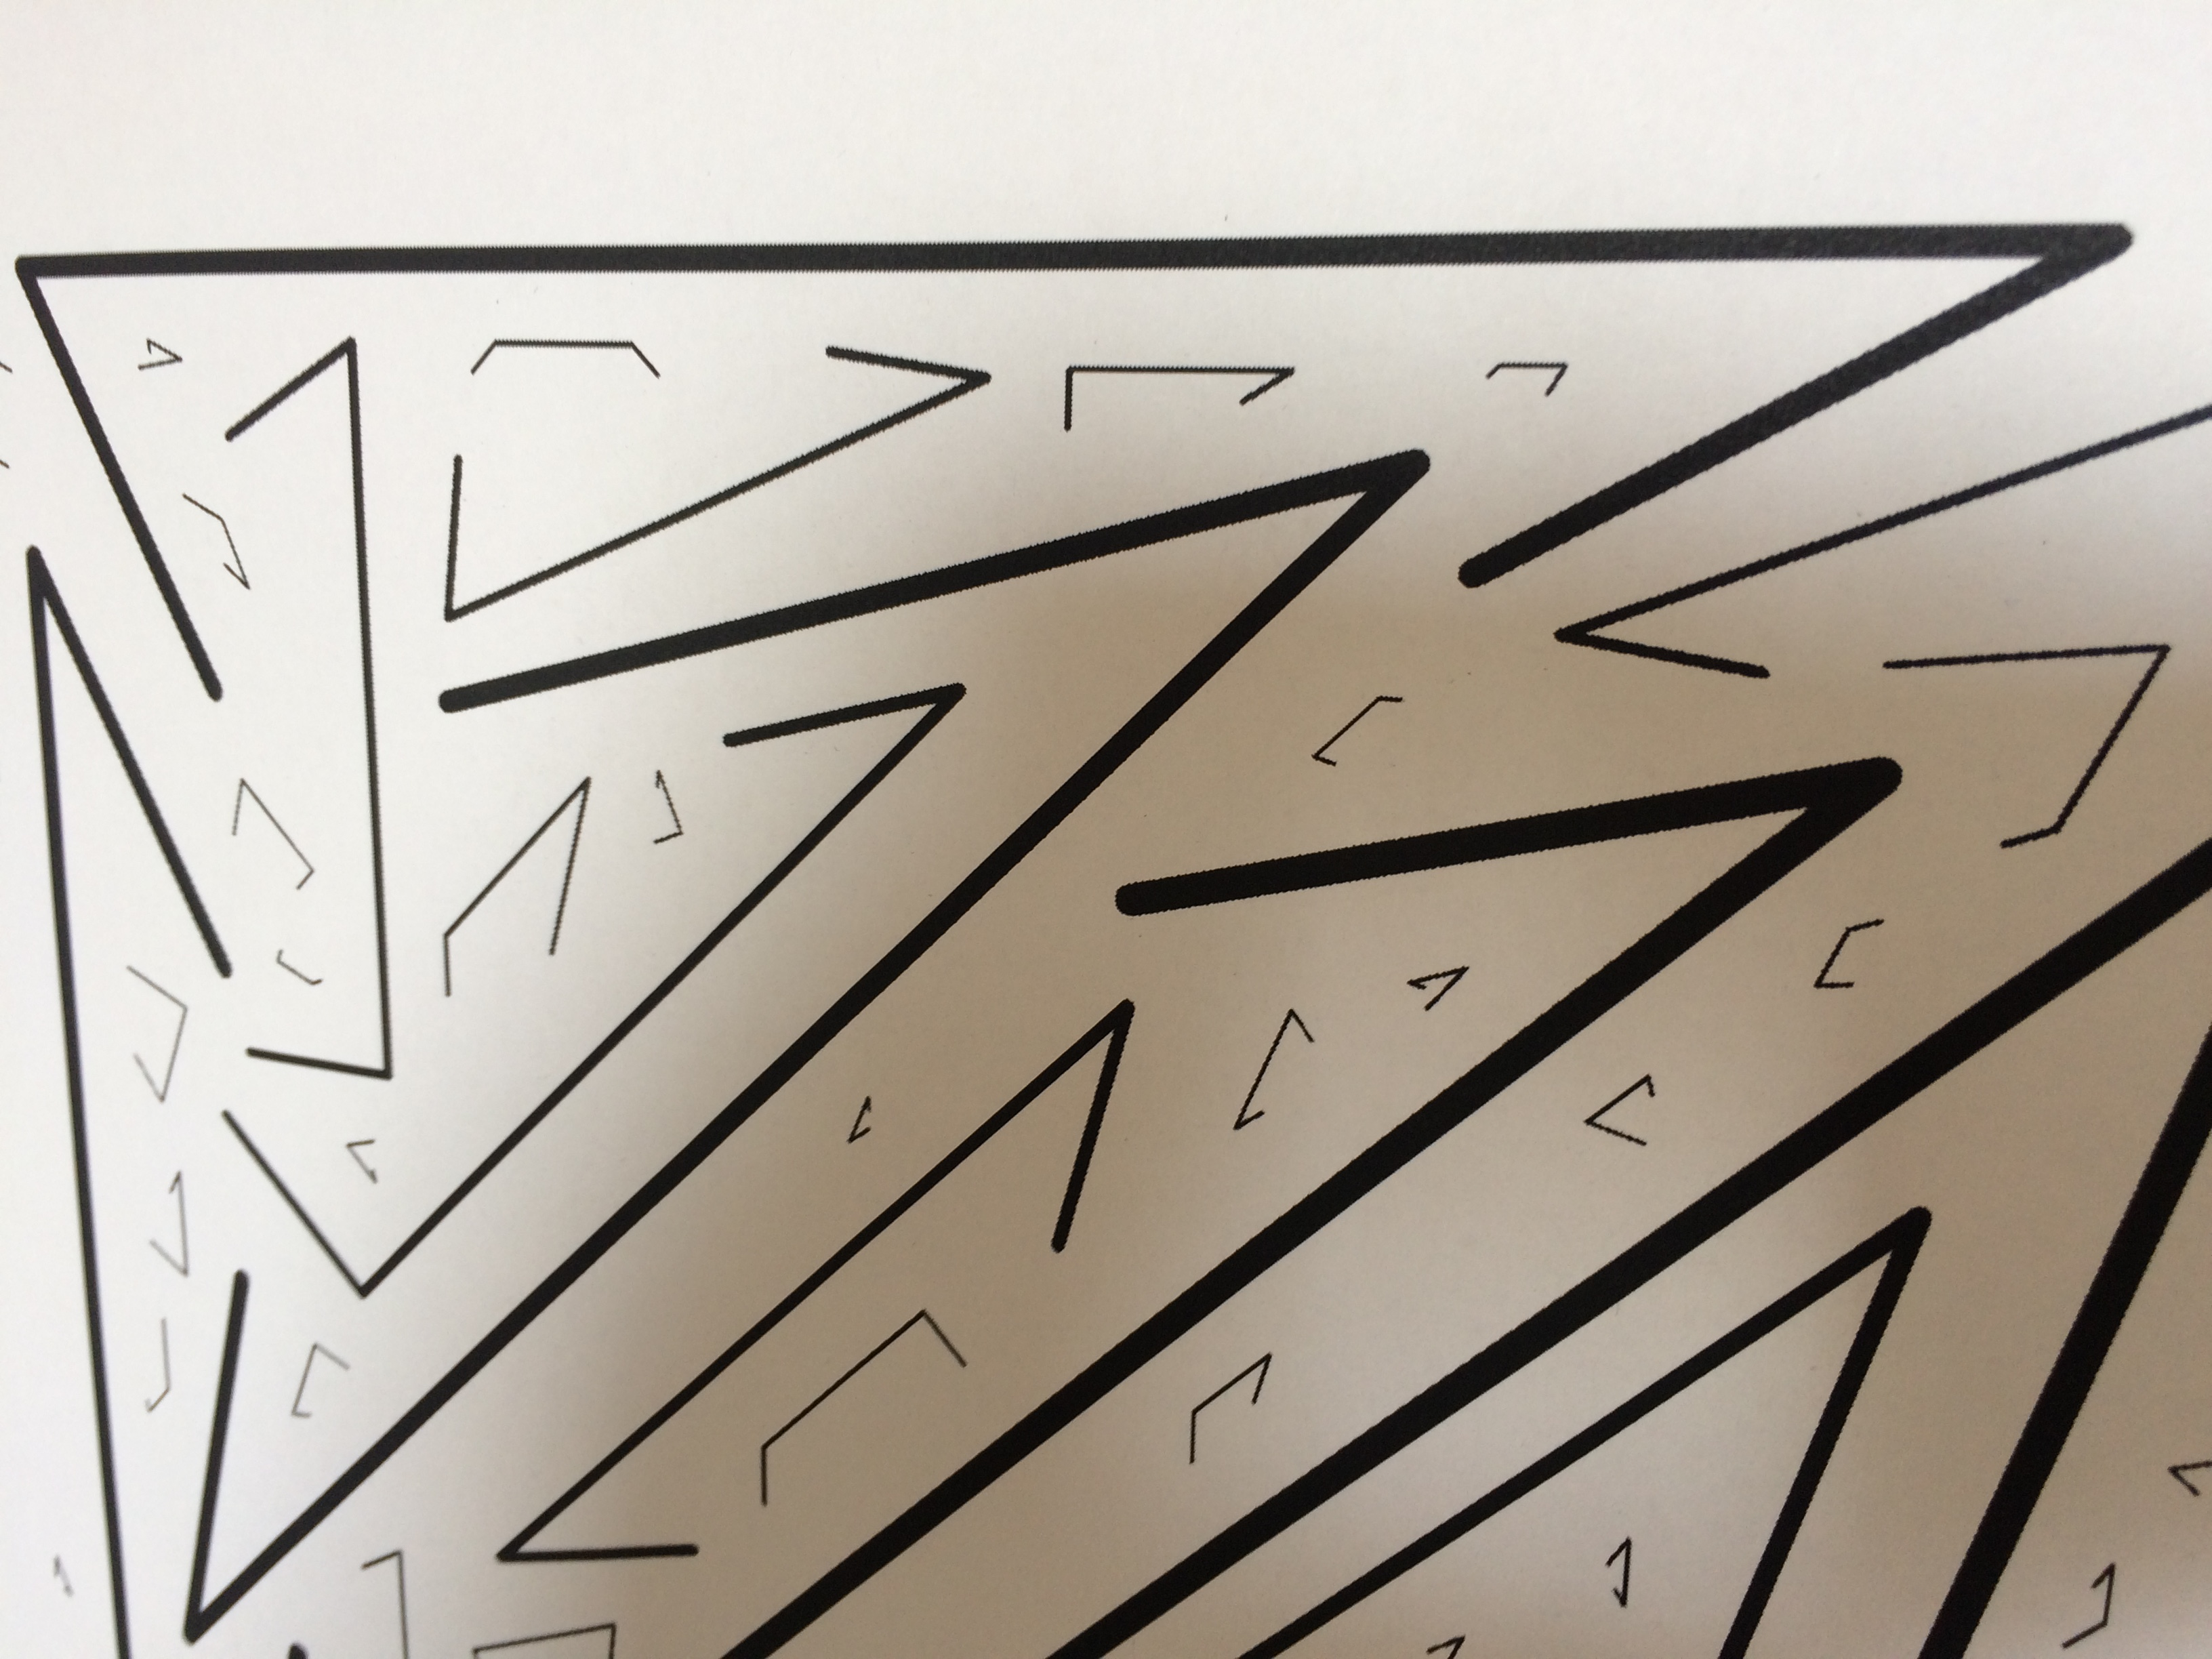
\includegraphics[width=0.75\textwidth]{figures/t35_01.JPG}
	\caption{Partially visible marker (taken with commercial smartphone)}
	\label{fig:partialMarkerShot}
\end{figure}
In this chapter will be a short summary of the algorithms used for testing and performance comparison.

%-----------------------------------------------------------------------------------------------
\section{Theoretical Overview}
%-----------------------------------------------------------------------------------------------

Before going over how the image processing algorithms were applied to achieve quad detection, a short theoretical overview of the used algorithms will be presented.
To solve the problem at hand (i.e. to detect quad instances on an image) multiple well known image processing algorithms were used.
For line detection two variants of the Hough transform (Standard\cite{houghThetaRho} and Probabilistic\cite{MATAS2000119}) and a fundamentally different algorithm, the \textbf{LSD} was used.
As mentioned before, not only solutions based on line detection were tried during the course of this work; corner detection methods were also tried.
The Harris corner detector\cite{Harris88alvey} and it's improved version the Shi-Tomasi detector\cite{Shi94goodfeatures} were compared.

Although the implementation of the aforementioned algorithms were provided by the OpenCV framework, it was far from unnecessary to understand how each algorithm works.
They show their optimal performance on differently conditioned inputs.
For example, corner detection works well on "raw" images, while the Hough-transform based solutions need edge images of skeletons to perform.
It was important to know the limitations of each solution.
All in all, the understanding of the inner workings of the algorithms used was helpful in choosing the "right tool for the job".

In this section there will be the theoretical overview of the above mentioned algorithms, with some historical context.
Their comparative advantages for this project will also be highlighted.

%-----------------------------------------------------------------------------------------------
\subsection{Hough transformation}
%-----------------------------------------------------------------------------------------------

One of the most commonly used methods for line detection on images is the Hough transform.
Over it's long history many publications have been made about it's applications, performance and improvements.

Originally it was developed by Paul Hough in 1959 and later patented in 1962\cite{houghPatent}.
It was intended to be used for machine analysis of bubble chamber photographs.
In it's modern form (with the $\theta-\rho$ parametrisation) was introduced in 1972 by Duda and Hart\cite{houghThetaRho}.
The transformation became popular in the image processing community after Ballard's article\cite{BALLARD1981111} about generalising the algorithm for detection of arbitrary shapes.
There were many optimised and improved variants of the transformation, however the basic concept remained the same.
In 1990 a publication\cite{XU1990331} introduced the Randomized Hough Transform, which was a fundamentally new approach to the algorithm with notable merits.
As opposed to the one-to-many mapping of the simple Hough transform, the randomised version uses a convergent many-to-one mapping when creating the parameter space.

In this work the Standard Hough Transform and one of it's optimised versions, the Progressive Probabilistic Hough Transform will be used.
The PPHT, although being probabilistic, doesn't belong to the class of randomised Hough transforms.
It uses the same one-to-many mapping as the SHT.
The OpenCV framework provides implementations for the SHT and the PPHT, which is one of the main reason why they were chosen for this project.

After this short historical overview the theory of the transformations will be discussed.

%-----------------------------------------------------------------------------------------------
\subsubsection{Standard Hough Transform}
%-----------------------------------------------------------------------------------------------

The transformation is used to find instances of a model on digital images.
The models are usually simple geometric shapes like lines, circles or ellipses.
The curves are described by their parameters, e.g. slope and intercept for a line, centre point and radius for a circle etc..
Every non-zero pixel\footnote{The transformation works on binary images} votes for the features it could be part of.
The number of votes is stored for every possible parameter combination.
Then a threshold is applied to the stored votes, and the remaining parameters are accepted as model instances.
	
At first Hough described the algorithm to lines, but later the method would be generalised to any analytic\footnote{The Generalised Hough Transform even extends to arbitrary shapes} curve or shape.
This theoretical overview is based on the example of line detection.
The process is the same for every analytic curve, the only difference is the parameter space's dimension.
The original patent\cite{houghPatent} used the slope-intercept representation of lines.
\begin{equation}
y = m*x + b
\end{equation}
In this case, the \emph{parameter space} is 2 dimensional and it's axes are $m$ and $b$.
Every point in the parameter space represent an image space line.
With this representation every non-zero pixel in the image space transforms into a line in the parameter space.
For a given $(x_0,y_0)$ pair \eqref{houghLineMB} gives the line in the parameter space. 
\begin{equation}
\label{eq:houghLineMB}
b = -x_0*m + y_0
\end{equation}
Collinear points in the image show up in the parameter space as intersecting lines.
The more lines intersect in a given $(m_0,b_0)$, the more likely it is the image contains the $y = m_0*x + b_0$ line.
The problem with this parametrisation is that the parameter space is unbounded along both axes.
Both intersect and slope can have values in the range of $(-\infty, \infty)$.
Duda and Hart\cite{houghThetaRho} proposed an alternative parametrisation, which turned out to be better for application.
They used the \emph{normal parametrisation} of a line, shown in \eqref{normalParams}.
\begin{equation}
	\label{eq:normalParams}
	\rho = x*cos(\theta) + y*sin(\theta)
\end{equation}
In \eqref{normalParams} $\rho$ means the distance of the line from the image plane's origin.
$\theta$ is angle of the normal vector of the line.
\begin{figure}[ht]
	\centering
	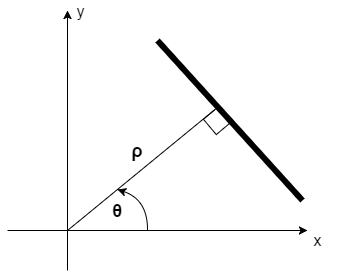
\includegraphics[width=0.5\textwidth]{figures/line_params.png}
	\caption{Normal line parameters}
	\label{fig:normalLineParams}
\end{figure}
If the \emph{normal parametrisation} is used the parameter space becomes finite in both dimensions.
$\theta$ is in the range of $(0,2\pi)$, $\rho$ is bounded by the image size.
In this case the image points define sinusoid curves in the parameter plane, and the line detection is done by searching for their intersections.
\begin{figure}[ht]
	\centering
	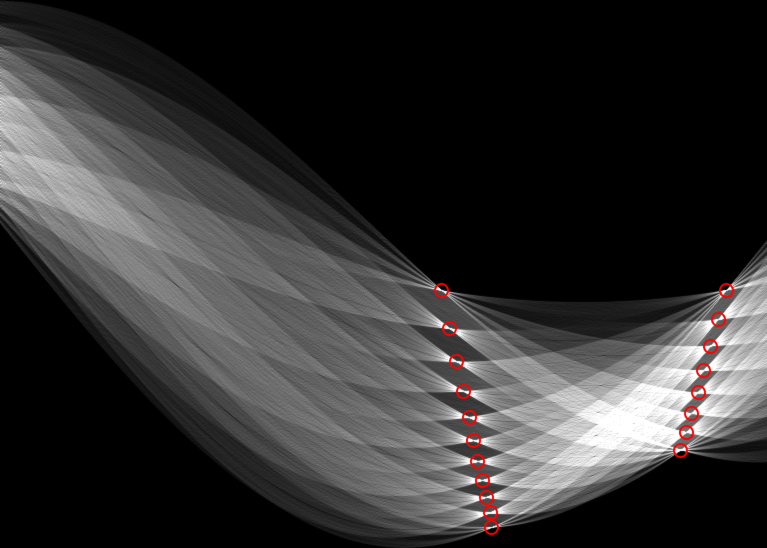
\includegraphics[width=0.6\textwidth]{figures/Perspective_chessboard_hough_transform.png}
	\caption{Hough-transform of a chessboard pattern}
	\label{fig:houghChessBoard}
\end{figure}

As mentioned before, the line detection is based on a voting scheme.
The parameter space (in this case a 2 dimensional plane) is divided into \emph{bins}.
$\rho$ and $\theta$ are quantised in the desired resolution.
The discrete $(\rho,\theta)$ pairs define the bins.
Every bin has accumulator.
When a given $(\rho_i,\theta_i)$ pair gets a vote it's corresponding accumulator is incremented by 1.
The \textbf{SHT} (Standard Hough Transform) uses one-to-many divergent mapping.
This means that every non-zero pixel votes for every possible parameter pair it could belong to.
The above mentioned sinusoid is calculated with the desired resolution for the pixel, and the corresponding accumulators are updated.

When the accumulation phase is completed for the whole image, the local maxima of the accumulators are found.
Usually a threshold is applied in order to reduce noise and eliminate too short line segments.
The radius of the non-maxima suppression also has impact on the results of the line fitting, it must be chosen carefully.
After this step the parameters for the most likely line candidates are available.

As the \textbf{SHT} does not provide the endpoints of the line, they must be found by examining the original binary image.
This can be done by simple checking every pixel along the line with the given parameters and deciding whether or not it is part of the feature.
If it is desired, lines with gaps can also be accepted with this method.
For more accurate fitting, a Least Squares approximation can also be applied to the pixels belonging to the line.

%-----------------------------------------------------------------------------------------------
\subsubsection{Progressive Probabilistic Hough Transform}
%-----------------------------------------------------------------------------------------------

The progressive probabilistic Hough transform is an optimised version of the SHT described in \cite{MATAS2000119}.
Probabilistic Hough transform variants were developed to overcome the comparatively high computational cost of the standard transform.
The core concept is the same for most probabilistic versions of the Hough transform: not every none-zero point votes, only a randomly selected subset.
These algorithms have to find a balance between minimising the proportion of image points that are used for voting while maintaining the accuracy of the detection process.

The original probabilistic Hough transform\cite{KIRYATI1991303} solved this issue by introducing a tunable parameter $p$ for the fraction of points to be used.
First, a $p$ fraction of the non-zero points are selected, than the SHT is performed on the selected subset.
$p$ can be low, the authors of \cite{KIRYATI1991303} presented successful experiments with $p=2\%$.
However, the results of the algorithm are greatly sensitive to the sampling rate.
The authors analysed the problem on the special case of a single line immersed in noise and tried to formulate a solution for determining the $p$ parameter.
They succeeded, but the practical applicability is severely limited\cite{MATAS2000119}: it requires \textit{a priori} knowledge of the number of points belonging to the line.
There was another approach to calculate the number of necessary votes\cite{BERGEN1991639}.
It was shown that the probabilistic Hough transform can be formulated as the Monte Carlo approximation of the SHT, thus it is possible to deduce the desired error rate using the theory of Monte Carlo evaluation.
Nevertheless, the core problem remained the same: \textit{a priori} information was necessary for determining the sampling rate parameter.
Usually there is only very limited information available, so conservative approximation is needed.
This leads to the calculation of more votes then necessary, thus reducing the main advantage of the probabilistic method.

The progressive probabilistic Hough transform solves the above issue by \textquote{exploiting the difference in the fraction of votes needed to reliably detect lines (features) with different number of supporting points}\cite{MATAS2000119}.
This way for long lines only a small fraction of the line's points have to vote for the line to be registered.
For shorter lines this proportion is of course higher.
For lines with supporting points close to the votes generated by background noise a full transform must be performed.

The authors of \cite{MATAS2000119} proposed the following algorithm to achieve the aforementioned goal.
At each iteration a random non-zero image point is selected for voting to the possible model instances it could belong to.
After each vote, the question \textquote{could the count be due to random noise?}\cite{MATAS2000119} is evaluated.
This requires a single comparison per bin update, with a threshold value changing by each vote cast.
When a model instance (line) is detected, the supporting points retract their votes.
The other points belonging to the same line are removed from the voting process.
The pseudo-code representation below is directly quoted from \cite{MATAS2000119}.

\begin{lstlisting}
1. Check input image, if it is empty then finish
2. Update the accumulator with a single pixel randomly selected from the 
   input image
3. Remove pixel from input image
4. Check if the highest peak in the accumulator that was modified by the 
   new pixel is higher than threshold l. If not then goto 1.
5. Look along a corridor specified by the peak in the accumulator, and find 
   the longest segment of pixels either continuous or exhibiting a gap not 
   exceeding a given threshold.
6. Remove the pixels in the segment from the input image
7. Unvote from the accumulator all the pixels from the line that have 
   previously voted.
8. If the line segment is longer than the minimum length add it into the 
   output list.
9. goto 1.
\end{lstlisting}

This algorithm has some considerable advantages of the standard and other, previous probabilistic variants of the Hough transform.
It eliminates the need of \textit{a priori} knowledge necessary for the tuning of probabilistic transforms while it remains much faster than the SHT.
It should detect every instance of a model detectable by the SHT, at the latest when the voting finishes with the same number of voted pixels as for the standard transform.
Another positive property of the algorithm is that features are detected as soon as the accumulator allows a decision: it is not necessary for all supporting points to vote.
The algorithm can also be terminated at any time and still provide some useful output\footnote{However this aspect is not really important for this project}.

Originally this transformation method was developed to speed up the Hough transform, while not being considerably more inaccurate.
However, an unexpected result was observed by the authors.
The PPHT outperformed the SHT in accuracy as well as speed.
In sample images consisting of randomly positioned equal length lines, the PPHT produced less false negatives (missed line segments) and less false positives (incorrectly detected lines).
This effect is due to the fact that PPHT clears out the votes of the detected lines as soon as they are found.
This reduces the clutter in the accumulator, resulting in more accurate results, while also being more computationally efficient.

It also worth noting that the PPHT could, in theory, use every enhancement that were developed for the SHT.
For example, the image gradient of the line segments could be used to reduce the number of pixels selected for voting.
However, this aspect was not researched in the boundaries of this project.

%-----------------------------------------------------------------------------------------------
\subsection{Line Segment Detector}
%-----------------------------------------------------------------------------------------------

A fundamentally different approach to line detection was described in \cite{LSDDet}.
The algorithm is named \textbf{LSD} - for Line Segment Detector - by it's creators.
It is which, unlike the SHT, detects line segments with subpixel accuracy by default.
The runtime of the process is linear in the pixel count of the processed image.
It also has fairly good noise suppression.
Another attractive property of the algorithm is that it doesn't have any parameters that require tuning by the user.
Every one of it's parameters are automatically tuned "under the hood".
Because of these advantageous properties was it considered for use in this project.
The implementation used was provided by the OpenCV framework.
In this section will be a short summary of the theory behind this algorithm.

The LSD takes as input a grayscale image and provides a list of line segments as output.
The line detection is based on the image gradient.
As a first step, a gradient field is generated from the input image.
The gradient is taken using a $2x2$ window, see \eqref{lsdGrad}.
\begin{equation}
	\begin{split}
		g_x = \frac{i(x+1, y) + i(x+1, y+1) - i(x,y) - i(x, y+1)}{2}, \\
		g_y = \frac{i(x, y+1) + i(x+1, y+1) - i(x,y) - i(x+1, y)}{2}
	\end{split}
	\label{eq:lsdGrad}
\end{equation}
Where $i(x,y)$ is the intensity of the grayscale image at $(x,y)$ point.
The magnitude of the gradient is calculated by \eqref{lsdGradMagn}.
\begin{equation}
	G(x,y) = \sqrt{g_x^2(x,y)+g_y^2(x,y)}
	\label{eq:lsdGradMagn}
\end{equation}
The algorithm uses the angle of the gradient, which will be referred to as LLA (level-line angle), and is calculated by \eqref{lsdGradAngle}.
\begin{equation}
	\arctan\Bigg(\frac{g_x(x,y)}{-g_y(x,y)}\Bigg)
	\label{eq:lsdGradAngle}
\end{equation}
The gradient obtained with \eqref{lsdGrad} is the image gradient at the point $(x+0.5, y+0.5)$.
This half pixel offset is later added to the endpoints of the detected line segments.

Using the gradient information, a level-line field is constructed.
\begin{figure}[ht]
	\centering
	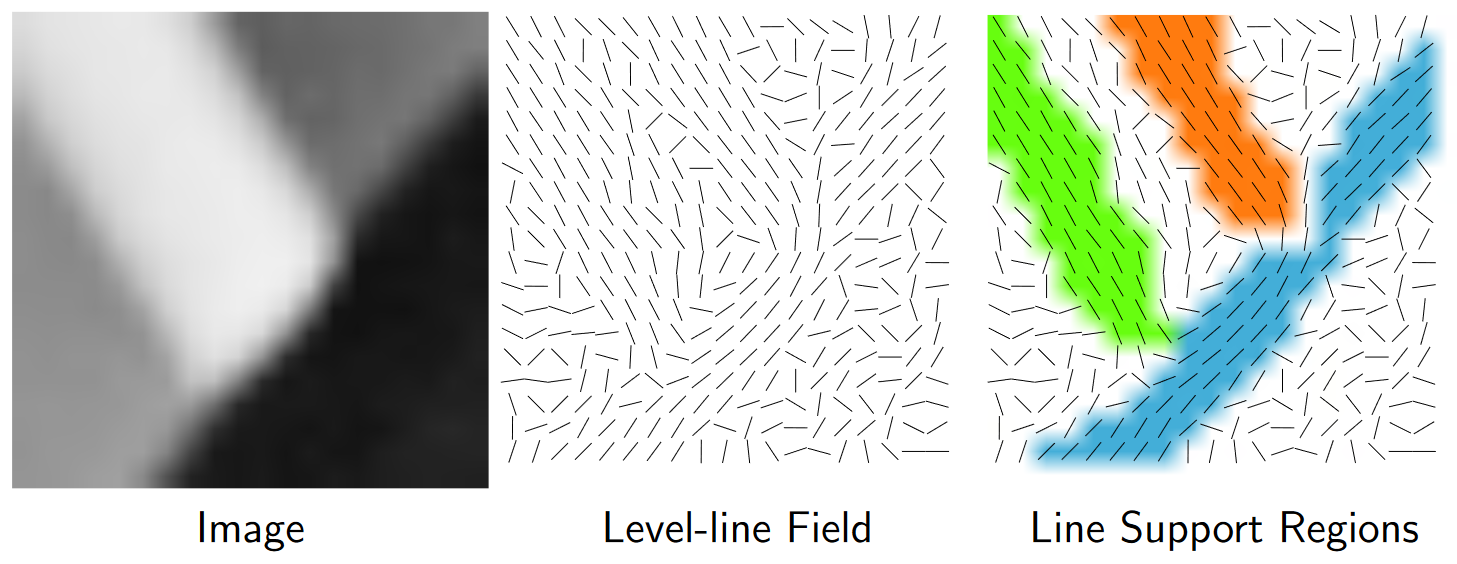
\includegraphics[width=0.75\textwidth]{figures/lsd_level_line_field.png}
	\caption{Illustration of the level-line field\cite{LSDDet}}
	\label{fig:lsdLevelLines}
\end{figure}
Figure \figref{lsdLevelLines} shows an example of the visualised level-line field.
The next step of the algorithm is the segmentation of this field.
It happens based on the level-line angle (the gradient angle defined in \eqref{lsdGradAngle}).
The pixels that have the same LLA within a given threshold are grouped together.
These segments are referred to as \textit{line support regions}, see figure \figref{lsdLevelLines} for illustration.
The segmentation is done with a region growing process.

Each \textit{line support region} is a candidate for a \textit{line segment}\cite{LSDDet}.
The line segments are represented with a rectangle.
The main direction of the rectangle is determined by the principal inertial axis of the \textit{line support region}.
The size of the rectangle is chosen in a way to cover the whole \textit{line support region}.

\begin{figure}[ht]
	\centering
	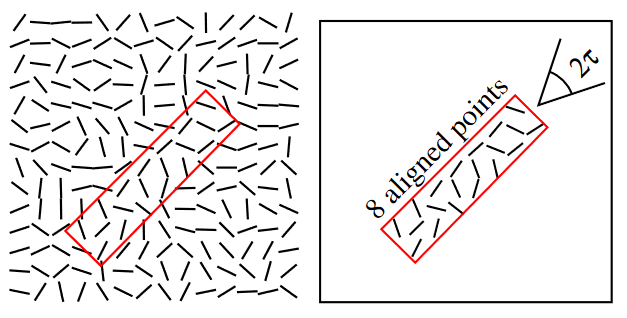
\includegraphics[width=0.75\textwidth]{figures/lsd_aligned_point.png}
	\caption{Illustration of the aligned points\cite{LSDDet}}
	\label{fig:lsdAligned}
\end{figure}
The pixels in the rectangle that have LLA close to the angle of the rectangle are called \textit{aligned points}\cite{LSDDet}.
Figure \figref{lsdAligned} shows an example for the rectangular representation and the \textit{aligned points}.
The \textit{aligned points} are used in the validation step of the algorithm.

The LSD algorithm uses an \textit{a contrario} validation method.
The idea behind that method is checking if it is probable that the current supporting points are caused by random noise.
To achieve this, the authors of \cite{LSDDet} created a noise model of the \textbf{level-line field}.
A \textit{line segment} becomes validated if the expected number of it's occurrences on the noise model is low\footnote{i.e. It is unlikely to be caused by random noise}.

The algorithm detects the sharp transients in the image gradient.
Technically, it detects edges.
A line on the image produces two line segments as output, for it's two light-dark transition.
The line segments detected by LSD are directional: the order of the endpoints of a line segments depend on the direction of the light-dark transition.

After this short summary of the algorithm\footnote{The description of the algorithm in pseudo-code form can be found in \cite{LSDDet}}, some of it's more interesting details will be described.

First off, the algorithm has a preprocessing step.
Before calculating the image gradient, the input image is downscaled to $80\%$ along both axes\footnote{or to $64\%$ of it's area}.
This is done to cope with aliasing and quantisation artefacts present in most images, for example the staircase effect.
The alternative to this subsampling would be the blurring of the image, however that would have some unfavourable side effects.
Blurring would affect the statistics of the \textit{a contrario} model.
Some structures would be detected in a blurred white noise image.
With a correct down-sampling the white noise statistics can be preserved.
The choice of scale factor was an optimum between filtering out noise and keeping valuable data.

Another interesting feature of the algorithm is the order in which the possible lines are processed.
LSD is a greedy algorithm, it tries to process the most significant edges first.
Pixels with higher gradient magnitude correspond to more contrasted edges.
In order to process the pixels with the highest contrast first, some ordering is needed.
However, most sorting algorithm require $O(n \log(n))$ operations.
To avoid this, LSD uses a pseudo ordering that can be done in linear time.
The interval between zero and the highest gradient magnitude in the image is divided into $1024$ equal bins.
Then each pixel is assigned to the bin corresponding to it's gradient magnitude.
The processing (region growing) is done first on the pixels selected from the bin containing the largest magnitudes.
$1024$ levels are enough to almost strictly order the gradients generated from a grayscale image with $256$ possible intensities.

To avoid unnecessary processing, a threshold is also applied to the gradient magnitudes.
Pixels with a low gradient represent flat regions or slowly changing intensities.
These pixels are marked and are not taking part in the later processing steps.
This threshold also helps reduce the effects of quantisation noise.	

The rectangular approximation of the line segment happens after the segmentation of the level-line field.
The rectangle is calculated based on the gradient magnitudes of the pixels belonging to a segment.
The gradient magnitude is viewed as the "mass"\cite{LSDDet} of the pixel, and the centre of the rectangle is the mass centre point of the segment.
The coordinates of the centre point are calculated by the formula given in \eqref{lsdTcpCord}
\begin{equation}
	\begin{split}
		c_x = \frac{\sum_{j \in Region} G(j) * x(j)}{\sum_{j \in Region} G(j)} \\
		c_y = \frac{\sum_{j \in Region} G(j) * y(j)}{\sum_{j \in Region} G(j)}
	\end{split}
	\label{eq:lsdTcpCord}
\end{equation}
Where $G(j)$ is the gradient magnitude of pixel $j$, calculated by \eqref{lsdGradMagn}.
$x(j)$ and $y(j)$ represent the $x$ and $y$ coordinate of point $j$, respectively.
The angle of the main rectangle is defined to be the principal inertial axis of the segment.
It can be calculated from the eigenvector of associated with the smallest eigenvalue of the matrix of \eqref{lsdMMat}.\cite{LSDDet}
\begin{equation}
	M =
	\begin{bmatrix}
		m^{xx} && m^{xy} \\
		m^{xy} && m^{yy}
	\end{bmatrix}
	\label{eq:lsdMMat}
\end{equation}
Where $m^{xx}, \dots$ is defined below.
\begin{equation}
	\begin{split}
		m^{xx} = \frac{\sum_{j \in Region} G(j) * (x(j) - c_x)^2}{\sum_{j \in Region} G(j)} \\
		m^{yy} = \frac{\sum_{j \in Region} G(j) * (y(j) - c_y)^2}{\sum_{j \in Region} G(j)} \\
		m^{xy} = \frac{\sum_{j \in Region} G(j) * (x(j) - c_x)(y(j) - c_y)}{\sum_{j \in Region} G(j)}
	\end{split}
\end{equation}

This is the short overview of the LSD algorithm, with some of it's more interesting nuances highlighted.
The full description is available in \cite{LSDDet}.

%-----------------------------------------------------------------------------------------------
\subsection{Corner Detection}
%-----------------------------------------------------------------------------------------------

Detecting quads not necessarily means the detection of line segments.
Along with the above described methods based on line detection, a corner detecting algorithm was also benchmarked.
The concept of this detection method is as follows.
Detect the corners and end-points of a quad with some corner detection algorithm.
Checks which detected pairs are connected with lines (or edges).
Based on the connected pairs and their ordering, a quad can be reconstructed.

The OpenCV framework provides implementations for some popular corner detection algorithms.
Specifically the Harris detector and the Shi-Thomas detector are covered.
In this section will be a short theoretical summary of corner detection in general, and some specifics of the above mentioned solutions.

The basic idea of most corner detection algorithm is the following.
Considering a local window on an image, corner regions show large change in average intensity if the window is shifted by a small amount in any direction.
The mathematical formulation of the following idea is shown in \eqref{moravec}.
$E_{x,y}$ is the change in intensity produced by shifting the window by $(x,y)$.
$I_{u,v}$ is the intensity of the image at the point $(u,v)$, and $w_{u,v}$ specifies the image window.
In the simplest case, the image window is rectangular and it is unity in a specified region and zero otherwise.

% Moravec corner measure
\begin{equation}
	E_{x,y} = \sum_{u,v} w_{u,v} | I_{x+u,y+v}-I_{u,v} |^2
	\label{eq:moravec}
\end{equation}

A naive approach of corner detection is to use \eqref{moravec} as it is.
The local maxima of the minimum of \eqref{moravec} above a certain threshold can be used for a metric.
With this method, three cases have to be considered:
\begin{enumerate}
	\item \textbf{Flat region:} The windowed image region has almost constant intensity. In that case, all shifts will show small change.
	\item \textbf{Edge region:} The windowed image region has an edge in it. In that case shift in one direction will result in large change, but shifts in other directions will show low change in intensity.
	\item \textbf{Corner region:} If the windowed region contains a corner, all shifts will show large change in the intensity.
\end{enumerate}

The shifts can be chosen in a couple of ways: $90^\circ$ shifts, $45^\circ$ shifts in 8 or 4 directions, etc...
Actually, this detection method is analysed in \cite{Harris88alvey}, and it is the base of the Harris detector.

\begin{figure}[t]
	\centering
	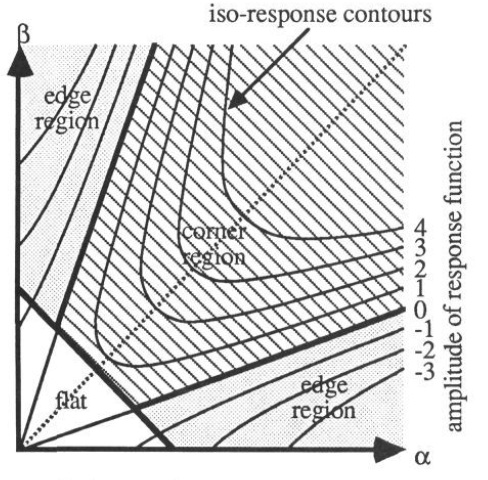
\includegraphics[width=0.75\textwidth]{figures/score-isoresponse-contours.jpg}
	\caption{Image point classification based on Harris measure\cite{Harris88alvey}}
	\label{fig:harrisMeasure}
\end{figure}

However, the the above described corner detector suffers from a number of problems\cite{Harris88alvey}.
Firstly, it provides an anisotropic response, as only a discrete set of shifts are used.
To address this issue, the Harris detector uses an analytic expansion of \eqref{moravec} around origin.
See \eqref{analyticHarris}.
\begin{equation}
	E_{x,y} = \sum_{u,v} w_{u,v} ( I_{x+u,y+v}-I_{u,v} )^2 = \sum_{u,v} w_{u,v} ( x \frac{\partial I}{\partial x} + y \frac{\partial I}{\partial y} + O(x^2,y^2))^2
	\label{eq:analyticHarris}
\end{equation}
Another problem is that the above detection method's response is noisy\cite{Harris88alvey} because of the rectangular and binary image window.
The Harris detector resolves this issue by using a circular and smooth (for example Gaussian) window:
\begin{equation}
	w_{u,v} = e^{- \frac{u^2 + v^2}{2\sigma^2}}
\end{equation}
The third issue Harris found with the use of \eqref{moravec} as a corner metric is that it responds too readily t edges\cite{Harris88alvey}.
This is because only the minimum of $E$ is taken into account when deciding whether a sampled window contains a corner or not.
To address this issue, a reformulation of the corner measure was proposed that takes the variation of $E$ with the direction of the change into consideration.
For small changes, $E$, the average change in intensity generated by a shift with $(x,y)$ can be written as:
\begin{equation}
	E(x,y) = (x,y) M (x,y)^T
\end{equation}
Where $M$ is composed of the image gradients in the window. \eqref{mMatrix} shows $M$ using the notation of \eqref{mMatrixNotation}
\begin{equation}
	I_x = \frac{\partial I}{\partial x}, I_y = \frac{\partial I}{\partial y}
	\label{eq:mMatrixNotation}
\end{equation}
\begin{equation}
\begin{bmatrix}
	I_x^2 && I_x I_y \\
	I_x I_y && I_y^2
\end{bmatrix}
	\label{eq:mMatrix}
\end{equation}

\begin{figure}[t]
	\centering
	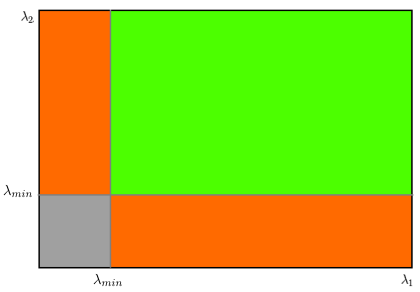
\includegraphics[width=0.75\textwidth]{figures/shitomasi_space.png}
	\caption{Image point classification based on Shi-Tomasi measure. Image source: OpenCV documentation}
	\label{fig:shiTomasiMeasure}
\end{figure}

Note that $M$ describes the shape of the local autocorrelation function's shape at the origin.
To describe $E$, \cite{Harris88alvey} uses the eigenvalues of the matrix $M$, as it provides a rotationally invariant description.
With this new method, the above mentioned cases (flat region, edge, corner) can be expressed as follows.
\begin{enumerate}
	\item \textbf{Flat region:} Both eigenvalues are small.
	\item \textbf{Edge region:} One eigenvalue of $M$ is small, the other is comparatively large.
	\item \textbf{Corner region:} Both eigenvalues are large.
\end{enumerate}
Figure \figref{harrisMeasure} shows the above defined regions with respect to the eigenvalues ($\alpha$ and $\beta$ are the eigenvalues of $M$).
The Harris detector also uses a metric for the "quality" of the detected edges or corners.
This is noted with $R$ and is defined below.
% Harris Measure
\begin{equation}
R = \det(M) - k(Trace(M))^2
\end{equation}
$k$ is a tunable parameter, its value is usually in the range of $0.01-0.05$.
The higher $R$ is, the more likely that a corner is present in the sampled window.
In figure \figref{harrisMeasure} the curves mark the regions in the $\alpha-\beta$ space that have the same $R$ value.

This is the short theoretical summary of the Harris detector.
A detailed mathematical derivation of the formulae can be found in \cite{Harris88alvey}.

The other corner detection method provided by the OpenCV framework is the Shi-Tomasi detector\cite{Shi94goodfeatures}.
This detector uses the same concept as the Harris detector, however uses a different measure to classify features as corners.
The scoring function is defined in \eqref{shiTomasiMeasure}. $\lambda_1, \lambda_2$ is the same as $\alpha, \beta$ for the Harris detector.
% Shi-Tomasi measure
\begin{equation}
	R = \min(\lambda_1, \lambda_2)
	\label{eq:shiTomasiMeasure}
\end{equation}
A feature is classified as a corner if $R$ is greater than a threshold $\lambda_{min}$.
Figure \figref{shiTomasiMeasure} shows this relation in the $\lambda_1-\lambda_2$ space.
The Shi-Tomasi measure, while being simpler and requiring less computational power, shows better performance in images\cite{Shi94goodfeatures}.

%-----------------------------------------------------------------------------------------------
\section{Application for Quad Detection}
%-----------------------------------------------------------------------------------------------

%-----------------------------------------------------------------------------------------------
\subsection{Conditioning}
%-----------------------------------------------------------------------------------------------

Before running the line detection algorithms some conditioning steps are done in order to improve their effectiveness.
These processes are not uniform - every fitting method needs it's own.

The Hough transformation traditionally works best on thin lines.
The easiest way is to generate an edge image with high-pass filtering.
The OpenCV framework offers a wide variety of features for this task.
The best result are obtained by using the Canny edge detector.

The skeletoning detector does not need a conditioning step, as it performs the band thinning on it's own.

The methods based on image gradients and corner detection both require some level of smoothing on the picture.
In case of the corner detection the smoothing is useful for removing the false positive matches caused by the jagged edges, or in case os JPEG images the artefacts caused by the compression.
The gradient detector simply gives a more spread-out and easier to analyse result on a smoothly changing gradient than it would on strict edge.
The smoothing is also implemented using the OpenCV framework, which provides easy access to Gaussian filtering.
The OpenCV implementation is based on convolution with a configurable Gaussian kernel.
The kernel size and the deviation in $x$ and $y$ direction can be set.
The Gaussian kernel and the convolution itself is handled in the framework.

%-----------------------------------------------------------------------------------------------
\subsection{LSD Quad Detector}
%-----------------------------------------------------------------------------------------------




%-----------------------------------------------------------------------------------------------
\section{Performance comparison}
%-----------------------------------------------------------------------------------------------

%-----------------------------------------------------------------------------------------------
\subsection{Test method}
%-----------------------------------------------------------------------------------------------

In this project multiple quad detection solutions are prototyped.
The best is needed to be selected.
It is not a trivial choice, as there are many criteria to be satisfied.
The algorithm needs to be accurate, robust, relatively fast, work on noisy images, etc...
Thorough testing is necessary to select the best algorithm for the task.
The tests should be reproducible and statistically relevant.
In this section will be a description of the testing method used in this project.

As a first step, a data source is necessary for the algorithms under test.
For this, randomly generated quads were used.
The random generator was constructed in a way that allowed some control over the generated data: the \textit{wuad size} and the range of the other parameters could be set.
To provide data for extensive testing, a large data set was generated.
Every algorithm received random quads with sizes ranging from $1\%$ to $75\%$ of the image size, in $1\%$ increments.
From each size 1000 quads were generated and provided to the detectors.
These values were chosen to cover a significant portion of the parameter space and to provide statistically significant results.

The generated quads were rendered by OpenCV and the generated images were the inputs for the detection algorithms.
The testing was done with images containing only a single quad.
There are many reasons for this.
First, it is important to limit the test scope.
In this step the quad detection was benchmarked. not the segmentation logic.
In the real use-case, the input image containing a marker is segmented, and the segments are fed to the quad detector separately.
The images were rendered with different levels of additive Gaussian White Noise.
The test series were run first on optimal images, and after that rerun with more and more added noise.
This was done to test the robustness.
Although the GWN covers only a small portion of the noise in a real image, these test did provide some insight.

The accuracy of the detection was analysed based on many different error measure.
Those are defined in the next section.
The experiments measured the expected value and the standard deviation of error of the algorithms.
These were plotted at the end of the test cycle.

The test method is summarised by the following pseudo-code program.
%test cycle in pseudo code
\begin{lstlisting}
quad_groups = empty_list
for size in [0.01:0.01:0.75]:
	group = generate_quads(count=1000, size=size)
	quad_groups.append(group)

error_series = empty_list
for group in quad_groups:
	pairs = empty_list
	for quad in group:
		img = render(quad)
		img = add_noise(img, noise_level)
		detected_quad = detector.detect_quad(img)
		pairs.append(quad, detected_quad)
	group_error = calculate_error(pairs)
	error_series.append(group_error)
display_result(error_series)	
\end{lstlisting}

The test framework, similarly to the tested algorithm, is implemented in python.

%-----------------------------------------------------------------------------------------------
\subsection{Error measure}
%-----------------------------------------------------------------------------------------------

In order to compare the performance of the quad detection algorithms some kind of scoring function is needed.
For this the use of detection error seems intuitive.
As a quad has 6 independent parameters, and these are stored in 2 different representations, defining an error measure is not straightforward.
Because of this, several scoring functions were defined during development, and many of those are actually used for comparing the algorithms.

As described in the previous section, the calculation of detection error is based on rendering a known quad and running the detection algorithms on it.
After the detection is done and it is successful\footnote{A quad instance is returned, which is not guaranteed}, some kind os measure is necessary to calculate the "distance" of the detected and the original quad.
Below will be the definitions the error measures used within this project to compare the quad detection algorithms.
The notations used in the formulae are listed here.
% notation
\begin{itemize}
	\item $Q^o, Q^d$: Original quad, detected quad
	\item $Q_p$: Parameter $p$ of quad $Q$, where $p$ can be any of the followings: $\{s, m_a, m_b, \alpha, \beta, \gamma\}$. 
	\item $C^o, C^d$: Corner set of the original and the detected quad
	\item $C_i^o, C_i^d$: The $i.$ corner of the original and the detected quad
	\item $C_{i,x}$: $x$ coordinate of the $i.$ corner of a quad
	\item $P^o, P^d$: the parameter space of the original and the detected quad. Using Section \sectref{quad}'s notation, it can be defined as $P = \{s, m_a, m_b, \alpha, \beta, \gamma\}$
\end{itemize}

As mentioned above, there are two different quad representations used\footnote{for details, see Section \sectref{quad}}.
One stores the coordinates of the corners, the other the quad parameters.
The most intuitive way for error calculation is based on the corner representation.
We can calculate the distance between the detected and the original corner.
\eqref{errAbsSumCoord}, \eqref{errAbsAvgCoord} and \eqref{errRelAvgCoord} define 3 scoring functions based on this idea. 
% sum of absolute position error
\begin{equation}
	E_{c,abs} = \sum_{1}^{4} \sqrt{(C_{i,x}^o - C_{i,x}^d)^2 + (C_{i,y}^o - C_{i,y}^d)^2}
	\label{eq:errAbsSumCoord}
\end{equation}
The first possibility is to calculate the sum of the distance between the detected and the original corners.
This naive approach has many drawbacks.
The main concern is that it does not take into account the \textit{size} of the quad.
The cumulation of error from every corner also distorts the results.
In reality, if every corner has some amount of noise in it's position, the quad parameter representation can still be quite close to the original.
However, if only one corner has a larger amount of error, the distortion will be much higher.
This error measure reports the same amount for both cases.
% avg absolute position error
\begin{equation}
	E_{c,avg} = \frac{1}{4} E_{c,abs}
	\label{eq:errAbsAvgCoord}
\end{equation}
The above points are also true is the average of the absolute displacements are used.

Better results can be achieved by using relative coordinate error.
The formula used by this work can be seen in \eqref{errRelAvgCoord}.
The problem of the error depending on the quad \textit{size} is solved by this.
As seen on the formula, the coordinate error is compared to the coordinates of the original quad corners.
% avg relative position error
\begin{equation}
	E_{c,rel} = \frac{1}{4}\sum_{1}^{4} \frac{\sqrt{(C_{i,x}^o - C_{i,x}^d)^2 + (C_{i,y}^o - C_{i,y}^d)^2}}{\sqrt{(C_{i,x}^o)^2 + (C_{i,y}^o)^2}}
	\label{eq:errRelAvgCoord}
\end{equation}
\eqref{errRelAvgCoord} was chosen for the comparison of algorithms based on the accuracy of corners detected.

The following scoring functions are based on the other quad representation.
This has considerable advantages compared to the corner based representation, because a much clearer picture of the distribution of error factors is obtained.
The quad parameters can be classified into 3 sets.
The is the quad size, which is an absolute length, measured in pixels.
Another category is formed of the angle parameters: the angle between the \textit{base} and each \textit{arm}, and the orientation (which is basically the angle between the \textit{base} and the image frame).
The third is the multiplier parameter.
These are not absolute lengths, they are calculated based on the base length.
Below will be proposed error measures for the three categories.

For the angle parameters, as a first approach an absolute error measure was defined.
As \eqref{errAbsSumAngle} shows, the 2 angle errors are summed.
As an alternative, their average also can be used.
Contrary to the coordinate errors, here the absolute angle error does not depend on the size of the quad.
These scoring functions can be useful if the absolute magnitude of the error is of interest.
% sum of absolute angle error
\begin{equation}
	E_{a,abs} = |Q_\alpha^o - Q_\alpha^d| + |Q_\beta^o - Q_\beta^d|
	\label{eq:errAbsSumAngle}
\end{equation}
% avg absolute angle error
\begin{equation}
	E_{a,avg} = \frac{1}{2} E_{a,abs}
	\label{eq:errAbsAvgAngle}
\end{equation}
Of course, relative error can also be defined for the angles, too.
See \eqref{errRelAvgAngle}.
This was used for comparison, because the relative values given as percentages were easier to evaluate.
% avg relative angle error
\begin{equation}
	E_{a,rel} = \frac{1}{2}\Bigg(\frac{|Q_\alpha^o - Q_\alpha^d|}{|Q_\alpha^o|} + \frac{|Q_\beta^o - Q_\beta^d|}{|Q_\beta^o|}\Bigg)
	\label{eq:errRelAvgAngle}
\end{equation}

The multipliers are very similar to the angles in terms of error metrics.
They describe a relative parameter, so the quad scale is not an issue here.
Nonetheless, both absolute and relative error measures were defined for completeness.
Similarly to the angles, both the sum os absolute errors and their average can be meaningful, depending on what is the goal of analysis.
% sum of absolute multiplier error
\begin{equation}
	E_{m,abs} = |Q_{ma}^o - Q_{ma}^d| + |Q_{mb}^o - Q_{mb}^d|
	\label{eq:errAbsSumMul}
\end{equation}
% avg absolute multiplier error
\begin{equation}
	E_{m,avg} = \frac{1}{2} E_{m,abs}
	\label{eq:errAbsAvgMul}
\end{equation}
For readability, the relative measure was chosen as a basis for comparison.
The values are normed with the respective parameter of the original (generated, thus it's parameters are known to an arbitrary level of precision) quad.
% avg relative multiplier error
\begin{equation}
	E_{m,rel} = \frac{1}{2}\Bigg(\frac{|Q_{ma}^o - Q_{ma}^d|}{|Q_{ma}^o|} + \frac{|Q_{mb}^o - Q_{mb}^d|}{|Q_{mb}^o|}\Bigg)
	\label{eq:errRelAvgMul}
\end{equation}

Orientation is handled differently from the other angle parameters.
This is due to two reasons.
First, it's conceptually different.
It describes a rotation as opposed to $\alpha$ and $\beta$ that describe angles between lines segments.
The second reason is mainly empirical: it turned out to be less error-prune than the other two.
% absolute orientation error
\begin{equation}
	E_{o,abs} = |Q_\gamma^o - Q_\gamma^d|
	\label{eq:errAbsOrient}
\end{equation}
% relative orientation error
\begin{equation}
	E_{o,rel} = \frac{|Q_\gamma^o - Q_\gamma^d|}{|Q_\gamma^o|}
	\label{eq:errRelOrient}
\end{equation}
Similarly to the previously discussed categories, the absolute and relative errors are defined.
Equations \eqref{errAbsOrient} and \eqref{errRelOrient} show the definitions.
For comparison, as before, the relative error was used.

The \textit{base length} or \textit{size} is the only absolute length parameter in this quad representation.
It makes sense to handle it separately, because many other parameters (orientation, arm multipliers) depend on it.
The scoring functions are defined below, similarly to the previous ones.
% absolute size error
\begin{equation}
	E_{o,abs} = |Q_s^o - Q_s^d|
	\label{eq:errAbsSize}
\end{equation}
% relative size error
\begin{equation}
	E_{o,rel} = \frac{|Q_s^o - Q_s^d|}{|Q_s^o|}
	\label{eq:errRelSize}
\end{equation}
For consistencies sake, also the relative error was used here for comparison.

The above defined error functions provide useful information if the distribution of error between the quad parameters is interesting.
However, this parametric quad representation lacks a scoring function that would provide information on the error magnitude as a whole.
To resolve this, one more error measure is proposed and used by this work.
The independent parameters of a quad can be viewed as coordinates in a 6 dimensional space.
The analogy stands, as the parameter space is a subset of $\mathbb{R}^6$.
A distance in that 6-dimensional space can be defined, see \eqref{errQuadSpaceDist}.
% distance in parameter space
\begin{equation}
	E_{sum} = \sqrt{\sum_{p \in P^o, q \in P^d} (p - q)^2}
	\label{eq:errQuadSpaceDist}
\end{equation}
This gives useful information about the absolute magnitude of error in the parametric quad representation.
Of course, the relative version of the above error measure can also be defined.
% distance in parameter space, relative
\begin{equation}
E_{sum, rel} = \frac{\sqrt{\sum_{p \in P^o, q \in P^d} (p - q)^2}}{\sqrt{\sum_{p \in P^o} p^2}}
\label{eq:errQuadSpaceDistRel}
\end{equation}
With this, a complete set of error measurement functions are defined.

It is reasonable to use both quad representations, thus both sets of error measures.
The corner representation is intuitive.
Also, as it is stated in the previous chapters of this work, the pose estimation algorithms use corresponding point pairs.
So the most relevant error component seems to be the one present in the quad corner coordinates, as it directly influences the accuracy of the calculated camera pose.

However, the two representations are equivalent.
It is possible to convert between the two without loosing useful information.
If discrete markers are used, with the parametric representation it is possible to further refine the detection results.
This can be done by replacing the detected quad with the closest known discrete one\footnote{This will be elaborated later on. This sentence is just to give a general idea and is not technically correct.}.
Currently this aspect of the marker is not implemented, it can be a subject of future improvements.

%-----------------------------------------------------------------------------------------------
\subsection{LSD Quad Detector results}
%-----------------------------------------------------------------------------------------------

\begin{figure}[t]
	\centering
	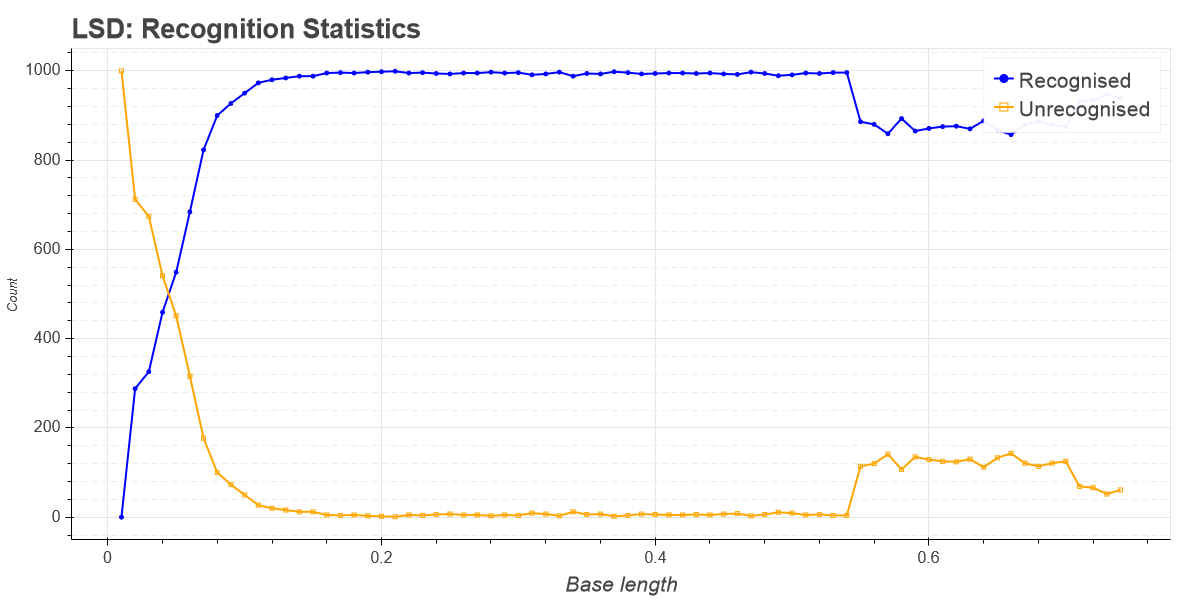
\includegraphics[width=0.9\textwidth]{figures/plots/lsd_rec_unrec_count.png}
	\caption{Recognised and unrecognised quads with respect to quad size, using the LSD method}
	\label{fig:lsdRecCnt}
\end{figure}
In this section the performance of the Line Segment Detector-based quad detection method will be evaluated.
Figure \figref{lsdRecCnt} shows the recognition count of the LSD quad detector.
Recognition fail is reported by the test framework if the detector couldn't find a quad on the input image or the average relative error is greater than $100\%$.
Detection failure can be caused by a couple of reasons within the algorithm.
If the quad on the image is too small, less than 3 lines may be detected.
The detector is helpless in this case, no quad is returned.
Another failure cause is connected to the small quads.
If the necessary number of line segments are detected, it is still possible for the detection to fail.
It can happen because a small quad rendered in comparatively low resolution looks more like a blob than connected line segments, thus the detected segments are not necessarily correspond to the segments of a quad.
These effects combined explain the rising edge in the beginning of the detected quad count on figure \figref{lsdRecCnt}.
\begin{figure}[t]
	\centering
	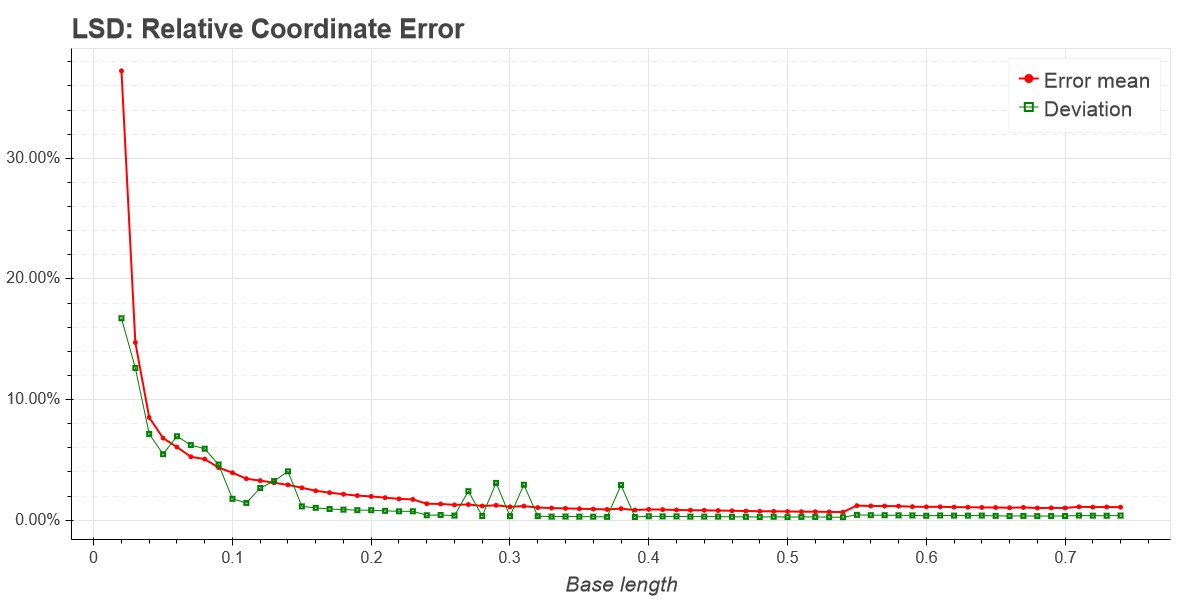
\includegraphics[width=0.9\textwidth]{figures/plots/lsd_relative_coordinate_error.png}
	\caption{Relative coordinate error with respect to quad size, using the LSD method}
	\label{fig:lsdRelCoordErr}
\end{figure}

\begin{figure}[ht]
	\centering
	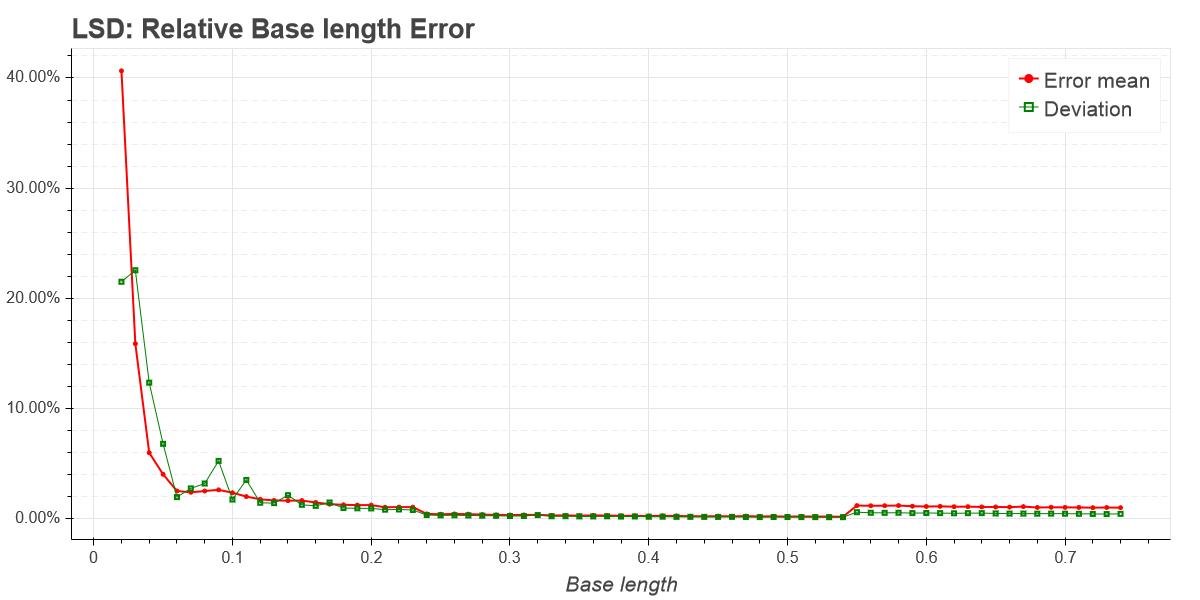
\includegraphics[width=0.9\textwidth]{figures/plots/lsd_relative_base_length_error.png}
	\caption{Relative base length error with respect to quad size, using the LSD method}
	\label{fig:lsdRelBaseErr}
\end{figure}
The sudden increase in the unrecognised count in the region of larger quads can be caused by a combination of two effects.
The quad rendering process is designed in a way that larger quads are rendered with thicker lines than the small ones.
This can cause issues with the merging of the two edges into one line.
The detector algorithm can be improved to better handle this.
The other part is that the LSD algorithm is sensitive to the scale of the features compared to the image size.
Detection can be improved if the algorithm is re-run on a down-sampled image.

\begin{figure}[ht]
	\centering
	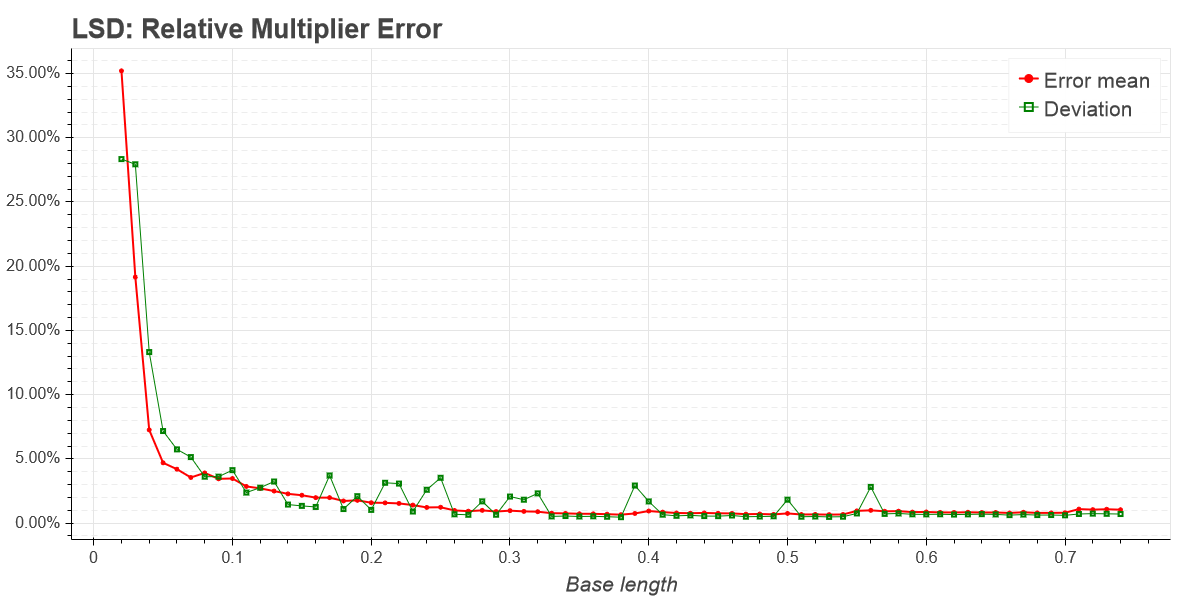
\includegraphics[width=0.9\textwidth]{figures/plots/lsd_relative_multiplier_error.png}
	\caption{Relative multiplier error with respect to quad size, using the LSD method}
	\label{fig:lsdRelMulErr}
\end{figure}
The overall performance of the LSD quad detector is quite good.
Figure \figref{lsdRelCoordErr} shows the average relative coordinate error and it's deviation as a function of the quad size.
This figure can be used as an indicator of the general performance the algorithm.
The relative coordinate error is below $5\%$ before the 0.1 scale factor is reached.
This means that the algorithm can detect quite small features relatively accurately.
In the optimal case, the average error is below $1\%$.
As the figure shows, the deviation of the error is also small, which indicates that the detection is stable.

\begin{figure}[ht]
	\centering
	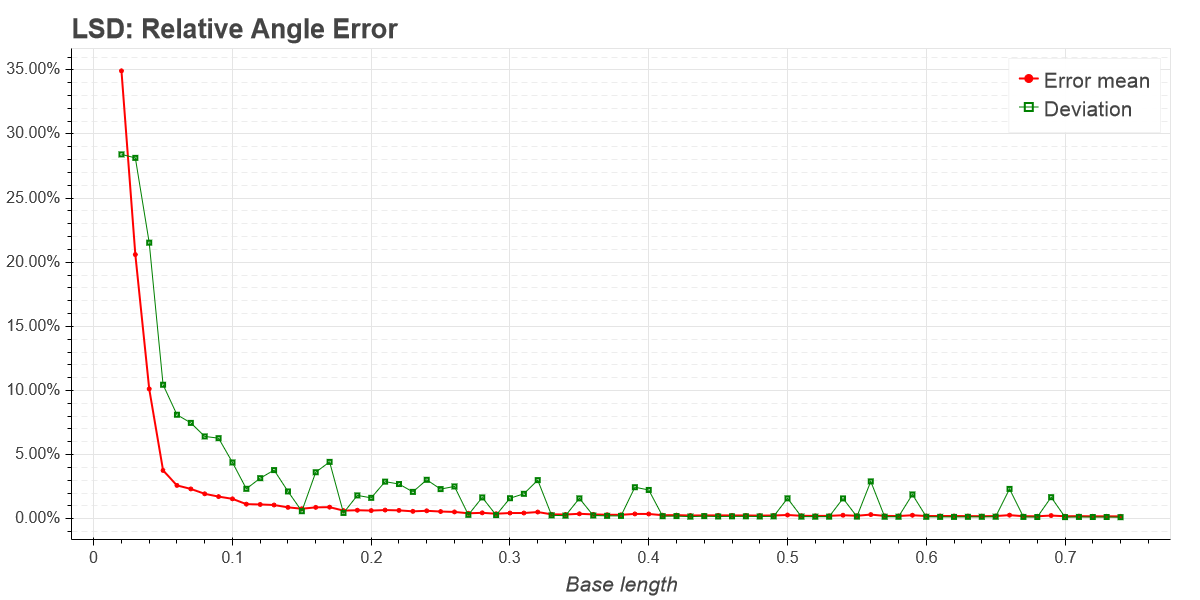
\includegraphics[width=0.9\textwidth]{figures/plots/lsd_relative_angle_error.png}
	\caption{Relative angle error with respect to quad size, using the LSD method}
	\label{fig:lsdRelAngleErr}
\end{figure}
The rest of the quad parameters show roughly the same level of accuracy.
The angle error (figure \figref{lsdRelAngleErr}) and the multiplier error (figure \figref{lsdRelMulErr}) stay below $5\%$ for most of the usable size range.

The error in the detected coordinates, base length, and multipliers show a small increase toward the region of larger quads.
This is caused by the same effect as causes the increase in recognition failure.
However, the angle parameters are not affected by this issue.
This is not unexpected, as the angle between lines is left unchanged by the offset caused by the line width. 

Another interesting observation can be made about the error distribution.
Figure \figref{lsdRelBaseErr} and \figref{lsdRelOrientErr} show a significantly smaller error level than the others.
Both the base length and the orientation only depends on the detection of the quad base, which is usually the largest feature of a quad.
This results in a more accurate detection, as more inliers are available for precise line detection.
The orientation is the most accurately detectable quad parameter. 
On top of it depending only on the quad base, it is unaffected by the error in the detection of the base length.
Only the angle of the line is important.
\begin{figure}[ht]
	\centering
	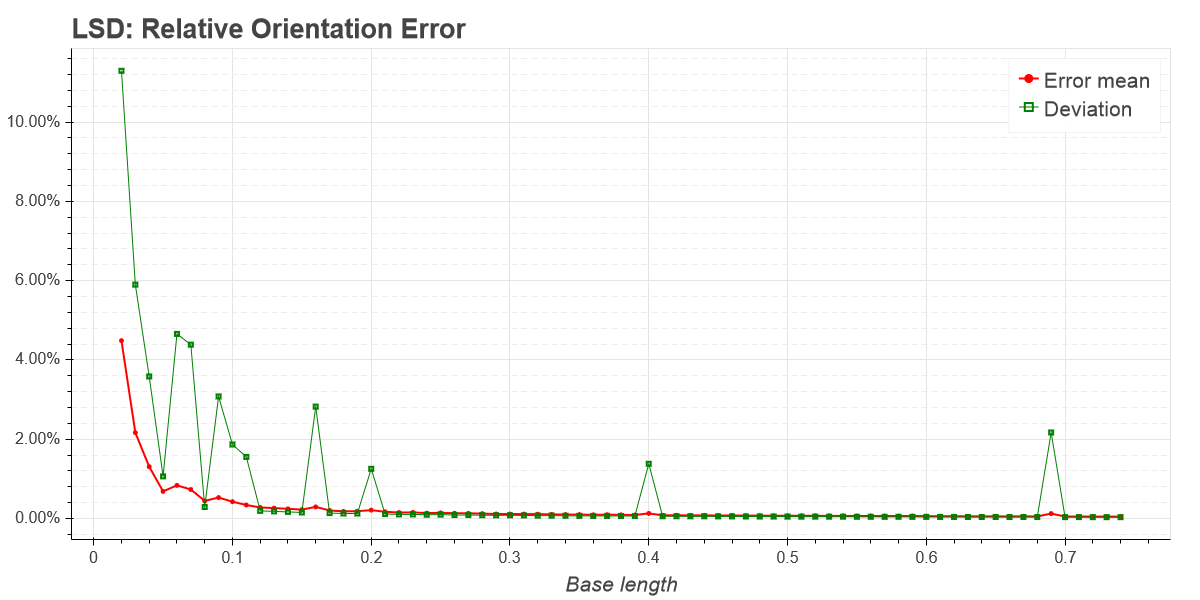
\includegraphics[width=0.9\textwidth]{figures/plots/lsd_relative_orientation_error.png}
	\caption{Relative orientation error with respect to quad size, using the LSD method}
	\label{fig:lsdRelOrientErr}
\end{figure}

\clearpage

%-----------------------------------------------------------------------------------------------
\subsection{SHT Quad Detector results}
%-----------------------------------------------------------------------------------------------

\begin{figure}[ht]
	\centering
	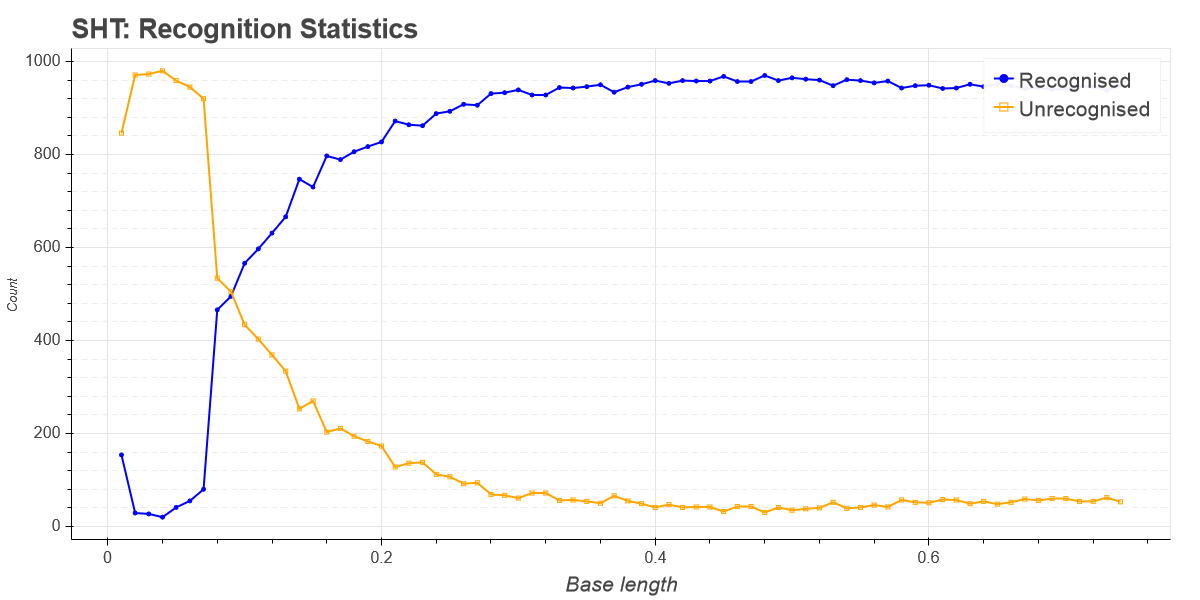
\includegraphics[width=0.9\textwidth]{figures/plots/sht_rec_unrec_count.png}
	\caption{Recognised and unrecognised quads with respect to quad size, using the SHT method}
	\label{fig:shtRecCnt}
\end{figure}

\begin{figure}[ht]
	\centering
	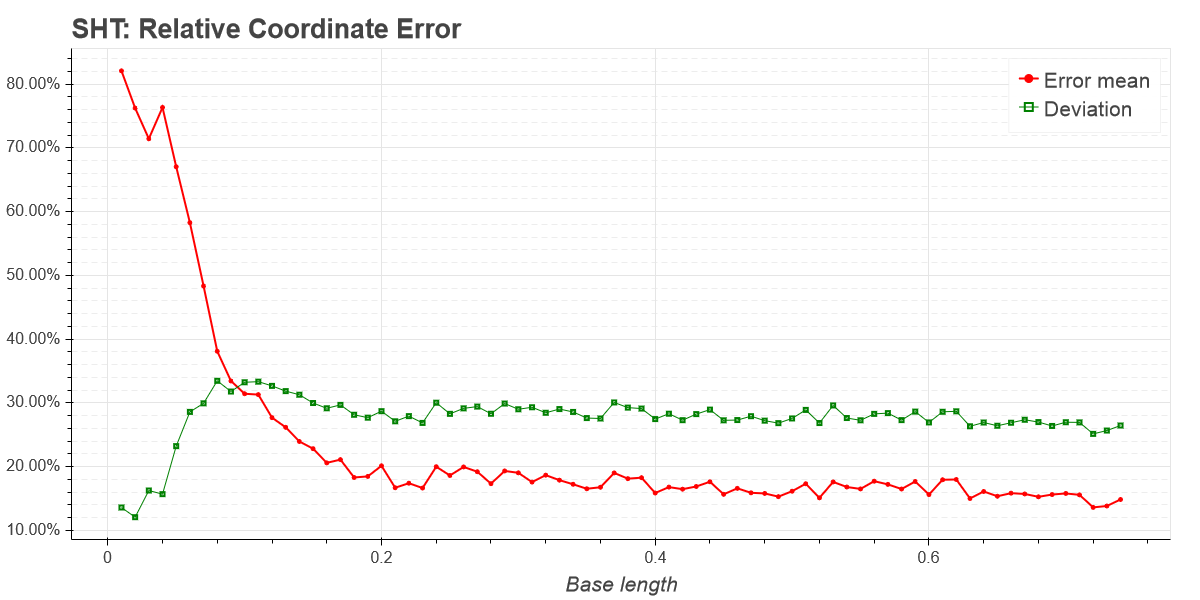
\includegraphics[width=0.9\textwidth]{figures/plots/sht_relative_coordinate_error.png}
	\caption{Relative coordinate error with respect to quad size, using the SHT method}
	\label{fig:shtRelCoordErr}
\end{figure}

\begin{figure}[ht]
	\centering
	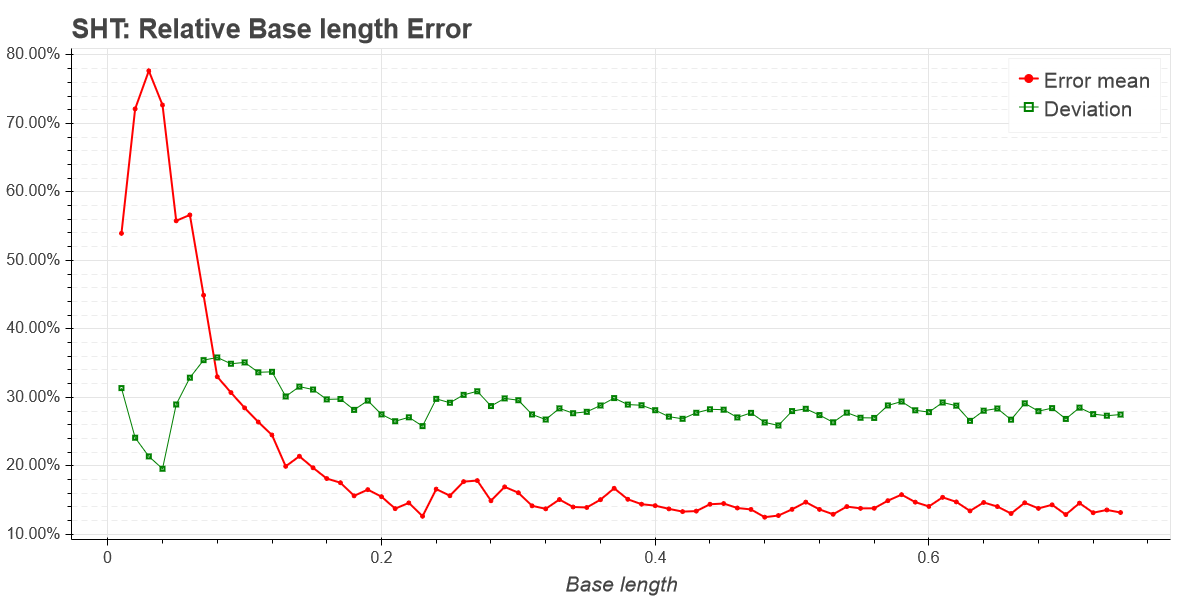
\includegraphics[width=0.9\textwidth]{figures/plots/sht_relative_base_length_error.png}
	\caption{Relative base length error with respect to quad size, using the SHT method}
	\label{fig:shtRelBaseErr}
\end{figure}

\begin{figure}[ht]
	\centering
	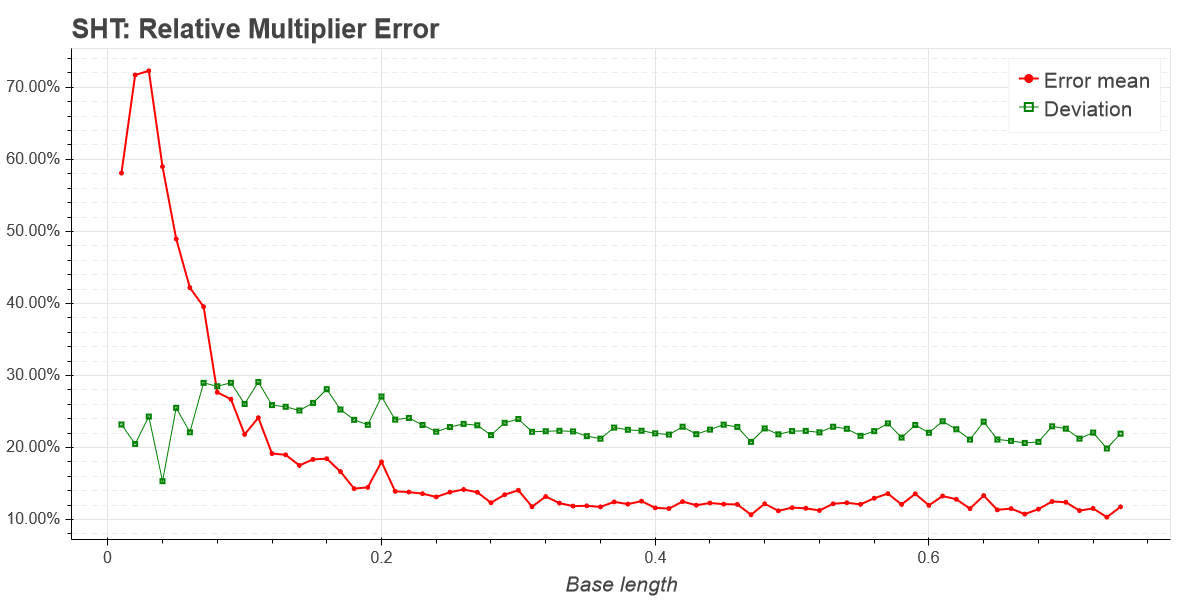
\includegraphics[width=0.9\textwidth]{figures/plots/sht_relative_multiplier_error.png}
	\caption{Relative multiplier error with respect to quad size, using the SHT method}
	\label{fig:shtRelMulErr}
\end{figure}

\begin{figure}[ht]
	\centering
	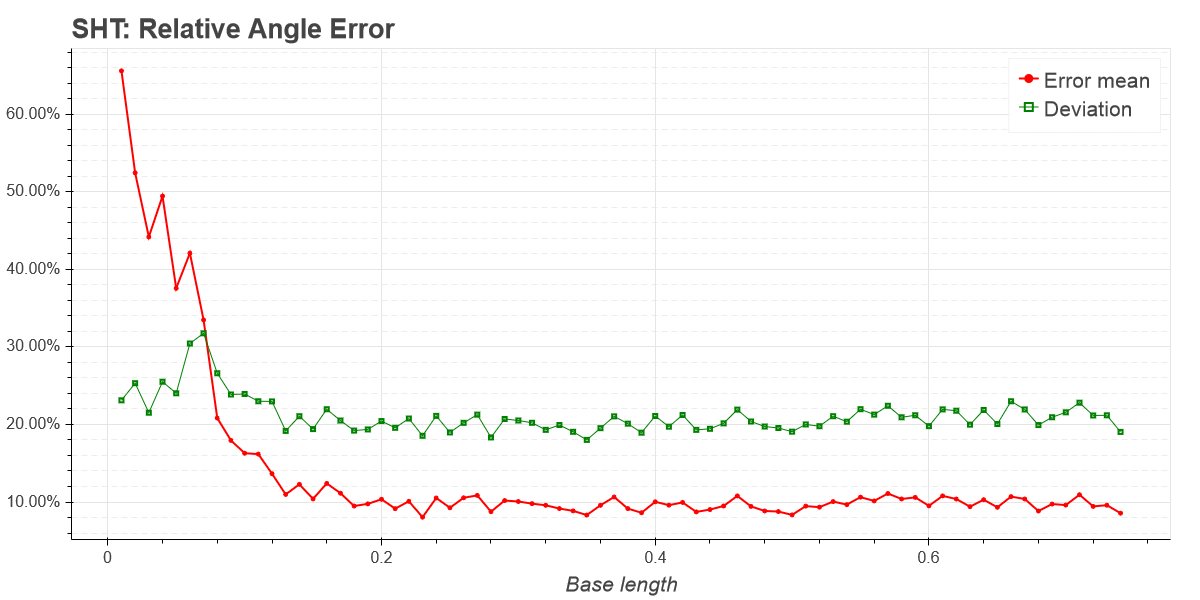
\includegraphics[width=0.9\textwidth]{figures/plots/sht_relative_angle_error.png}
	\caption{Relative angle error with respect to quad size, using the SHT method}
	\label{fig:shtRelAngleErr}
\end{figure}

\begin{figure}[ht]
	\centering
	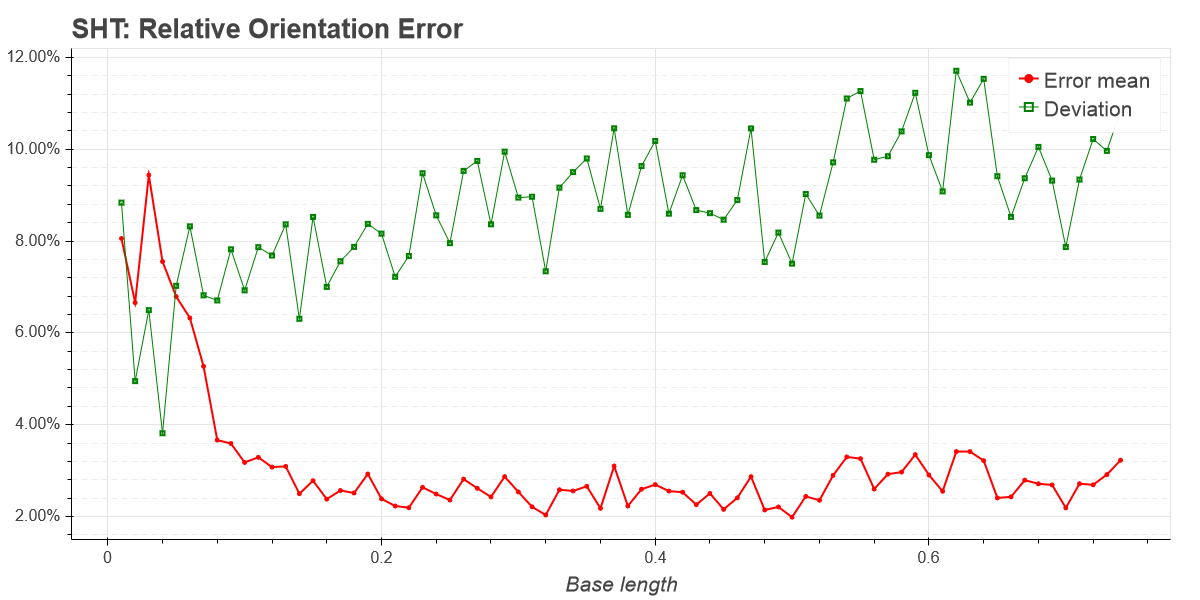
\includegraphics[width=0.9\textwidth]{figures/plots/sht_relative_orientation_error.png}
	\caption{Relative orientation error with respect to quad size, using the SHT method}
	\label{fig:shtRelOrientErr}
\end{figure}

\clearpage

%-----------------------------------------------------------------------------------------------
\subsection{PHT Quad Detector results}
%-----------------------------------------------------------------------------------------------

\begin{figure}[ht]
	\centering
	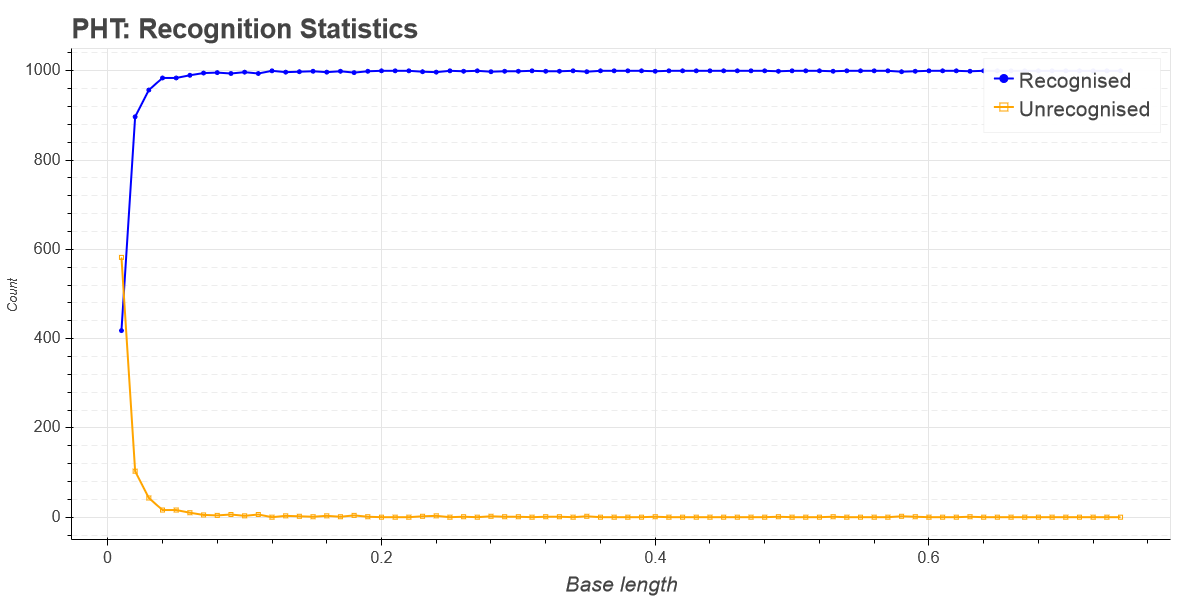
\includegraphics[width=0.9\textwidth]{figures/plots/pht_rec_unrec_count.png}
	\caption{Recognised and unrecognised quads with respect to quad size, using the PHT method}
	\label{fig:phtRecCnt}
\end{figure}

\begin{figure}[ht]
	\centering
	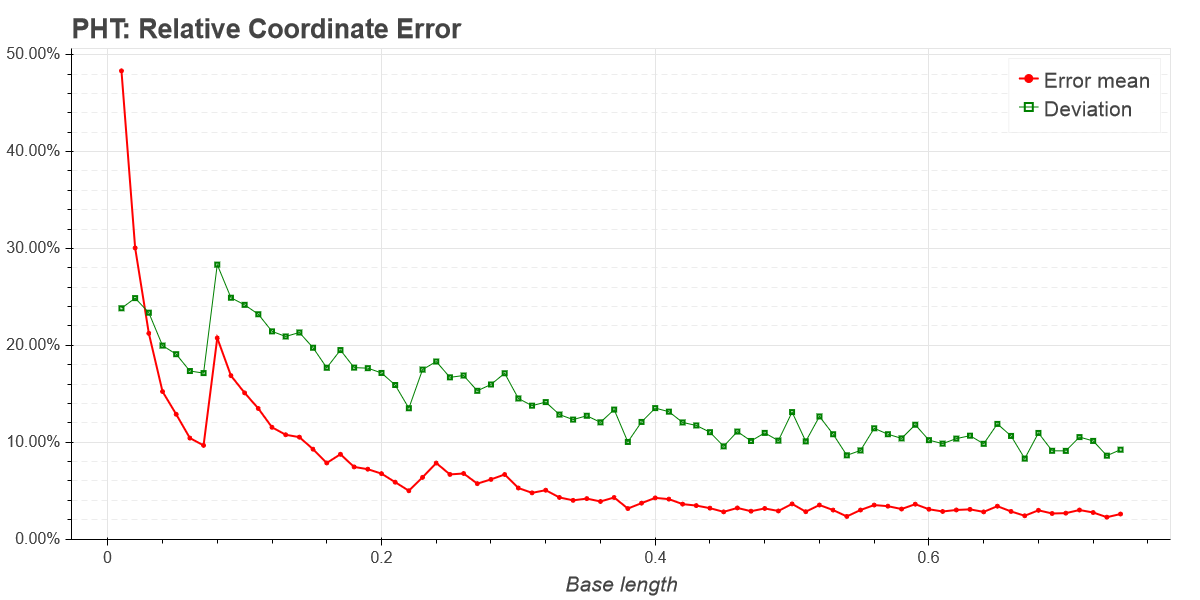
\includegraphics[width=0.9\textwidth]{figures/plots/pht_relative_coordinate_error.png}
	\caption{Relative coordinate error with respect to quad size, using the PHT method}
	\label{fig:phtRelCoordErr}
\end{figure}

\begin{figure}[ht]
	\centering
	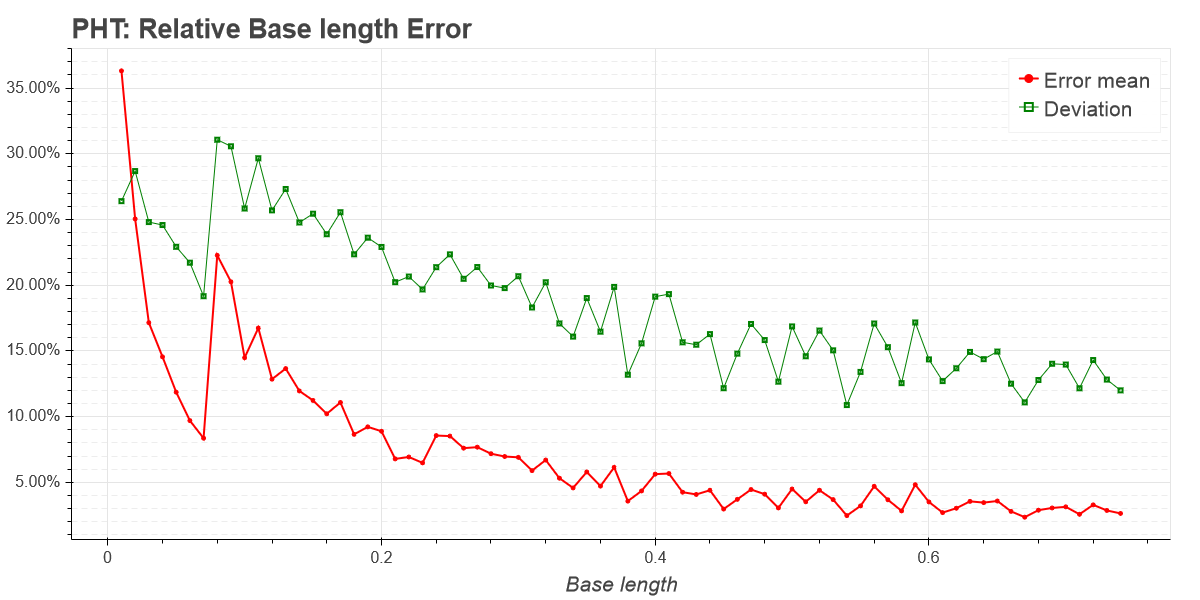
\includegraphics[width=0.9\textwidth]{figures/plots/pht_relative_base_length_error.png}
	\caption{Relative base length error with respect to quad size, using the PHT method}
	\label{fig:phtRelBaseErr}
\end{figure}


\begin{figure}[ht]
	\centering
	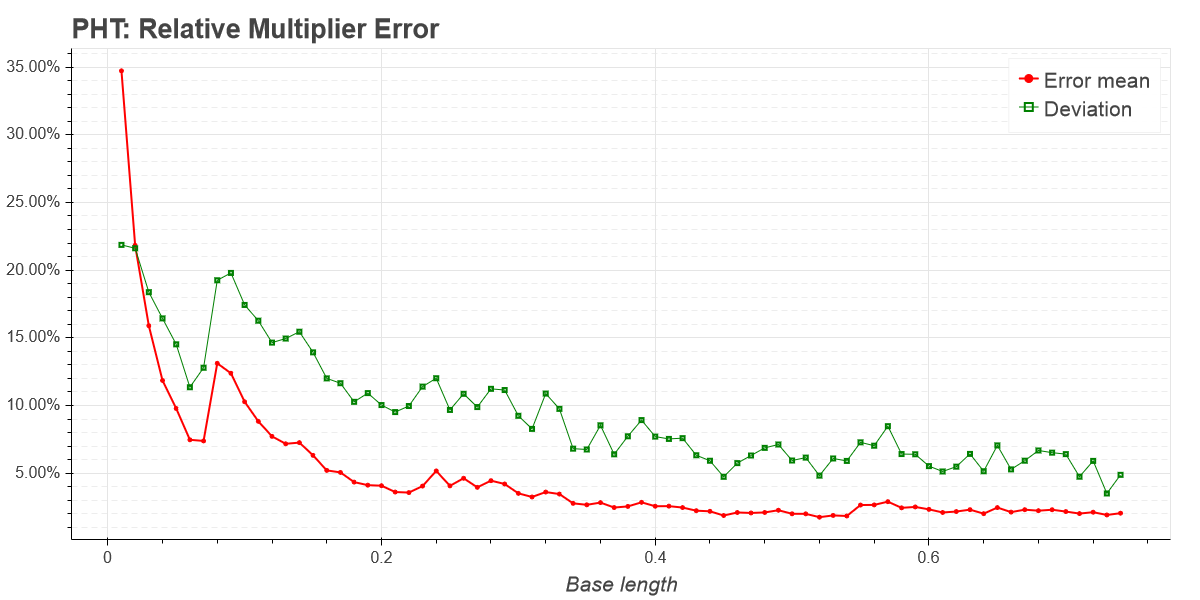
\includegraphics[width=0.9\textwidth]{figures/plots/pht_relative_multiplier_error.png}
	\caption{Relative multiplier error with respect to quad size, using the PHT method}
	\label{fig:phtRelMulErr}
\end{figure}

\begin{figure}[ht]
	\centering
	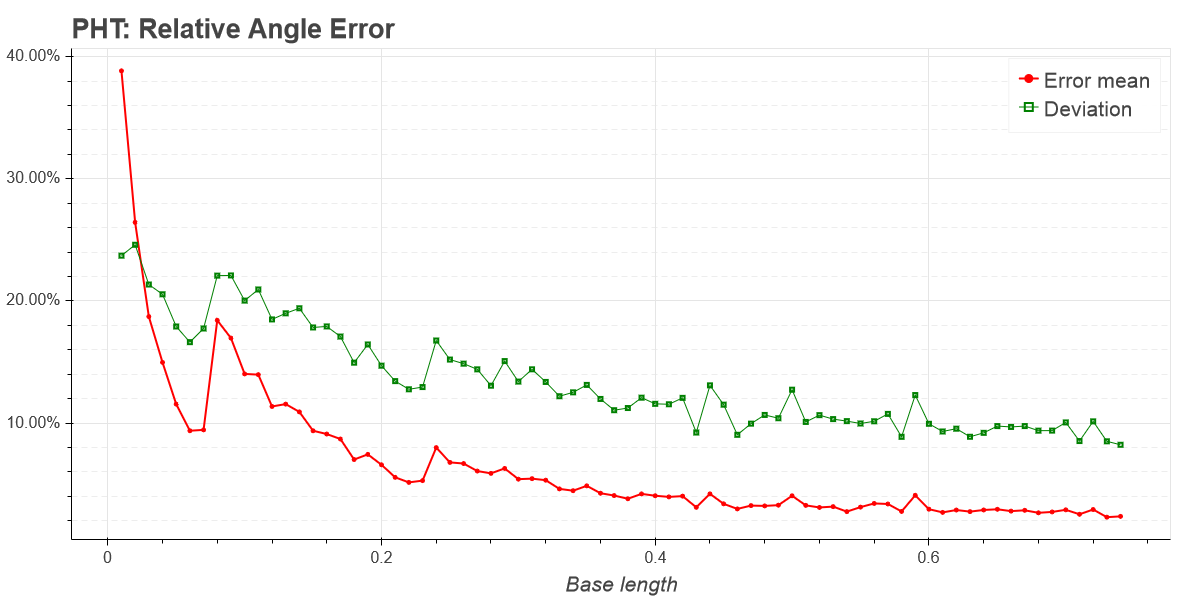
\includegraphics[width=0.9\textwidth]{figures/plots/pht_relative_angle_error.png}
	\caption{Relative angle error with respect to quad size, using the PHT method}
	\label{fig:phtRelAngleErr}
\end{figure}

\begin{figure}[ht]
	\centering
	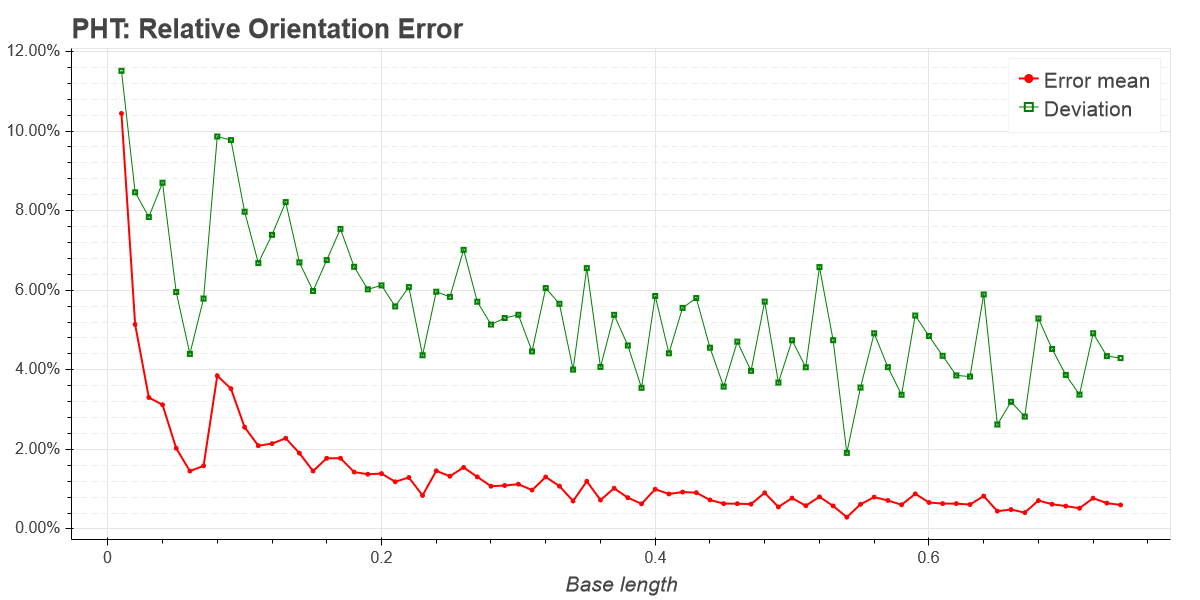
\includegraphics[width=0.9\textwidth]{figures/plots/pht_relative_orientation_error.png}
	\caption{Relative orientation error with respect to quad size, using the PHT method}
	\label{fig:phtRelOrientErr}
\end{figure}

\clearpage

%-----------------------------------------------------------------------------------------------
\subsection{Corner Quad Detector results}
%-----------------------------------------------------------------------------------------------

\begin{figure}[ht]
	\centering
	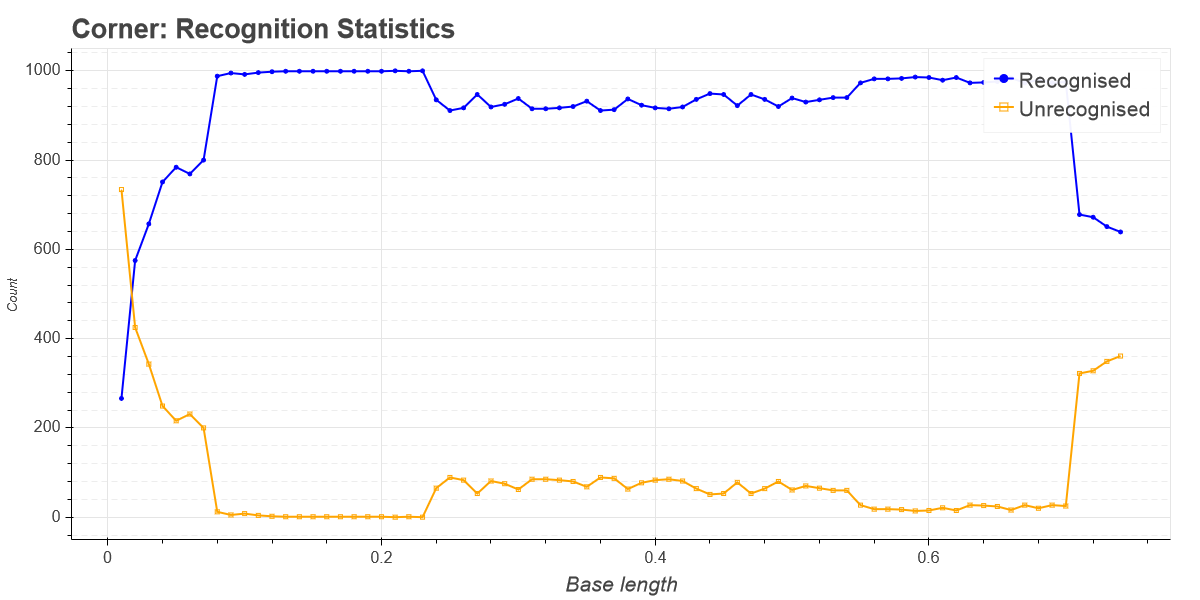
\includegraphics[width=0.9\textwidth]{figures/plots/corner_rec_unrec_count.png}
	\caption{Recognised and unrecognised quads with respect to quad size, using the Corner method}
	\label{fig:cornerRecCnt}
\end{figure}

\begin{figure}[ht]
	\centering
	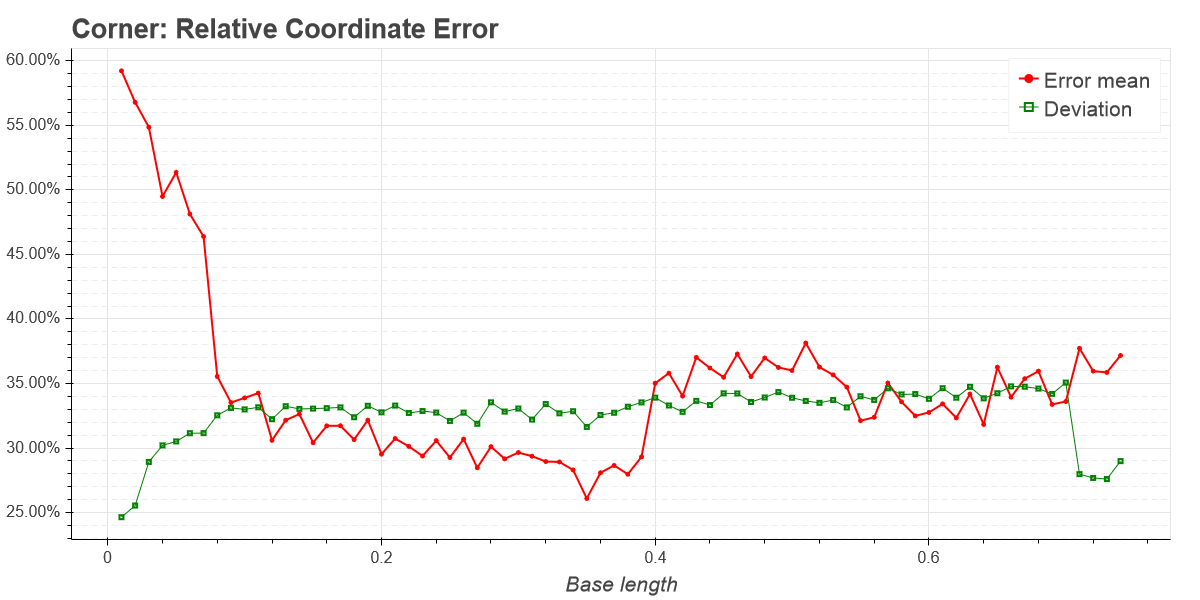
\includegraphics[width=0.9\textwidth]{figures/plots/corner_relative_coordinate_error.png}
	\caption{Relative coordinate error with respect to quad size, using the Corner method}
	\label{fig:cornerRelCoordErr}
\end{figure}

\begin{figure}[ht]
	\centering
	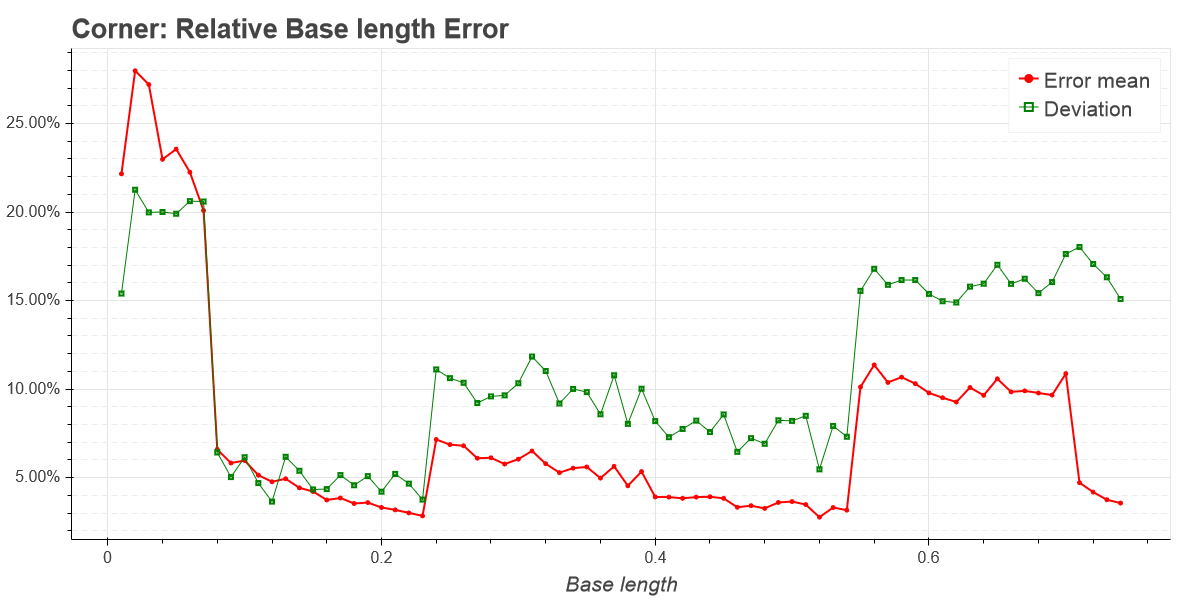
\includegraphics[width=0.9\textwidth]{figures/plots/corner_relative_base_length_error.png}
	\caption{Relative base length error with respect to quad size, using the Corner method}
	\label{fig:cornerRelBaseErr}
\end{figure}

\begin{figure}[ht]
	\centering
	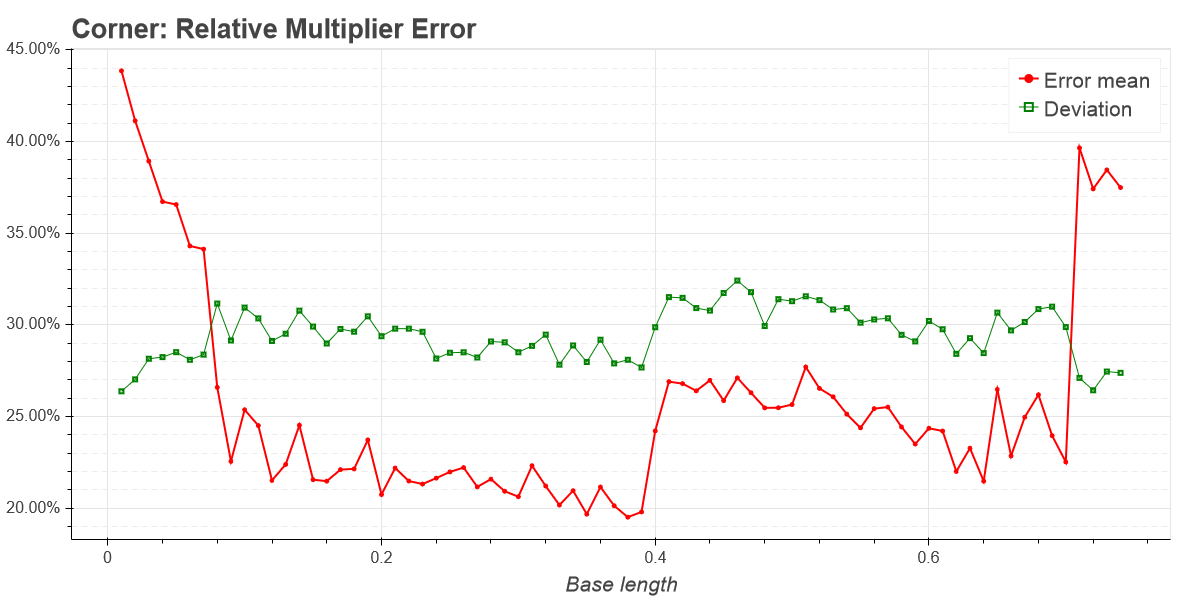
\includegraphics[width=0.9\textwidth]{figures/plots/corner_relative_multiplier_error.png}
	\caption{Relative multiplier error with respect to quad size, using the Corner method}
	\label{fig:cornerRelMulErr}
\end{figure}

\begin{figure}[ht]
	\centering
	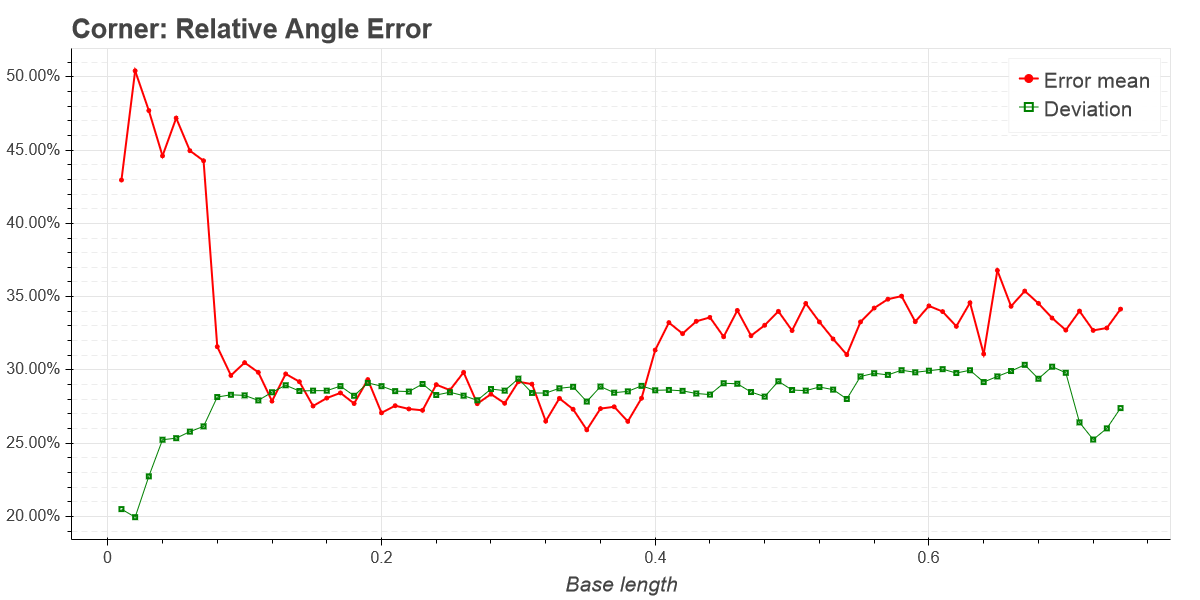
\includegraphics[width=0.9\textwidth]{figures/plots/corner_relative_angle_error.png}
	\caption{Relative angle error with respect to quad size, using the Corner method}
	\label{fig:cornerRelAngleErr}
\end{figure}

\begin{figure}[ht]
	\centering
	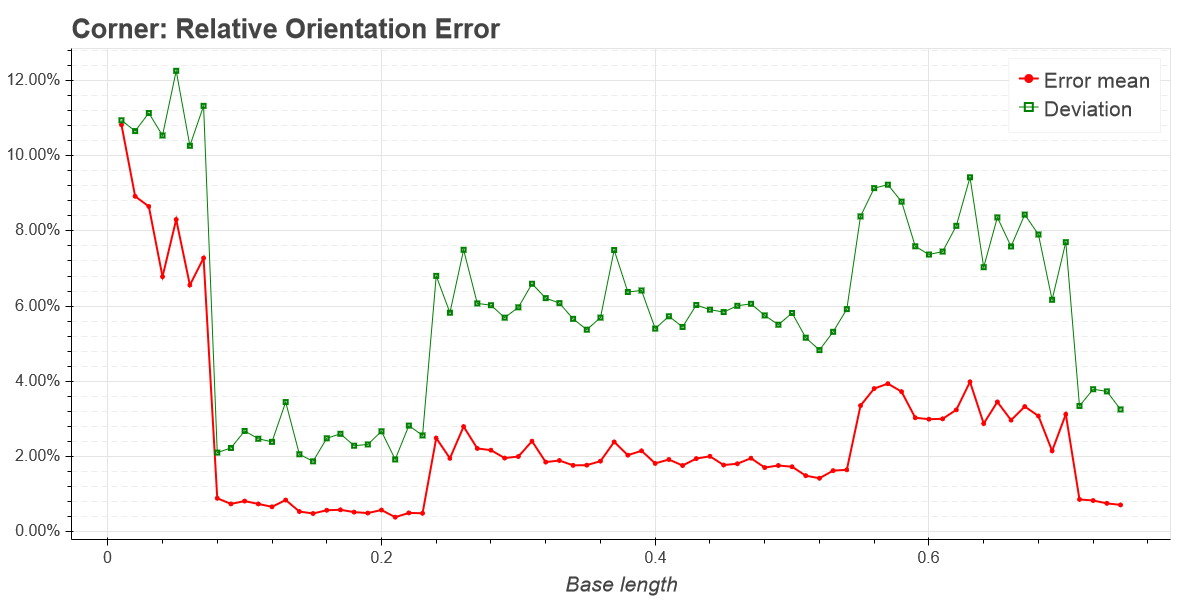
\includegraphics[width=0.9\textwidth]{figures/plots/corner_relative_orientation_error.png}
	\caption{Relative orientation error with respect to quad size, using the Corner method}
	\label{fig:cornerRelOrientErr}
\end{figure}

\clearpage

%-----------------------------------------------------------------------------------------------
\subsection{Summary}
%-----------------------------------------------------------------------------------------------